\documentclass[12pt,twoside]{report}
\usepackage{fullpage}

%Packages

%%%%%%%%%%%%%
%Bibliography stuff
\usepackage[utf8]{inputenc}
\usepackage[english]{babel}
\usepackage{csquotes}
\usepackage[
sorting=nyc,
backend=biber, %backend to use
style=authoryear, %citation style
uniquelist=false,
natbib,
block=ragged,
maxcitenames=2,
maxbibnames=99]{biblatex}


%manually enumerate the bibliography even if using author-year
% \defbibenvironment{bibliography}
%   {\begin{enumerate}}
	%   {\end{enumerate}}
%   {\item}

% Use last name, initial. unless this is non-unique. If this is non-unique, use full first name.
%From https://tex.stackexchange.com/a/631580
\DeclareNameFormat{always-init}{%
	\ifnumequal{\value{uniquename}}{2}
	{\usebibmacro{name:family-given}
		{\namepartfamily}
		{\namepartgiven}
		{\namepartprefix}
		{\namepartsuffix}}
	{\usebibmacro{name:family-given}
		{\namepartfamily}
		{\namepartgiveni}
		{\namepartprefix}
		{\namepartsuffix}}%
	\usebibmacro{name:andothers}}



\DeclareNameAlias{author}{always-init}
\DeclareNameAlias{editor}{always-init}

\ExecuteBibliographyOptions{useprefix=true}
\DeclareSortingNamekeyTemplate{
	\keypart{\namepart{family}}
	\keypart{\namepart{prefix}}
	\keypart{\namepart{given}}
	\keypart{\namepart{suffix}}}


%Sort by name-year-cite order (biblatex default is to sort by name-year-title).
\DeclareSortingTemplate{nyc}{
	\sort{
		\field{presort}
	}
	\sort[final]{
		\field{sortkey}
	}
	\sort{
		\field{sortname}
		\field{author}
		\field{editor}
		\field{translator}
		\field{sorttitle}
		\field{title}
	}
	\sort{
		\field{sortyear}
		\field{year}
	}
	\sort{\citeorder}
}

%Clear some things I do not want going into the bibliography
%from https://tex.stackexchange.com/a/89848
\AtEveryBibitem{\clearfield{month}}
\AtEveryBibitem{\clearfield{day}}
\AtEveryBibitem{\clearfield{url}}
\AtEveryBibitem{\clearfield{urlyear}}
%\AtEveryBibitem{\clearfield{note}}


%%%%%%%%%%%%%%%%
%Add a new command for citing things with possesive apostrophe. For example, if I want to write:  Smith's (2023) big idea, the apostrophe needs to go after the author but before the year
%From https://tex.stackexchange.com/a/537765
%The relevant command is \posscite
\DeclareNameWrapperFormat{labelname:poss}{#1's}

\newrobustcmd*{\posscitealias}{%
	\AtNextCite{%
		\DeclareNameWrapperAlias{labelname}{labelname:poss}}}

\newrobustcmd*{\posscite}{%
	\posscitealias
	\textcite}

\newrobustcmd*{\Posscite}{\bibsentence\posscite}

\newrobustcmd*{\posscites}{%
	\posscitealias
	\textcites}
%%%%%%%%%%%%%%%%%%%%%%%%%%%%%%%%%%%%%%%%%%%%%%%%%%

\usepackage{ragged2e} %for justifying text

\usepackage{amsthm, amsmath, amssymb} % Mathematical typesetting
\usepackage{mathrsfs} %fancy fonts for sigma-algebras
\usepackage{physics} %some physics symbols
\usepackage{float} % Improved interface for floating objects
\usepackage{newfloat} % Declare your own custom floats
\usepackage{graphicx, multicol} % Enhanced support for graphics
\usepackage{xcolor} % Driver-independent color extensions
\usepackage{framed}
\usepackage[normalem]{ulem} %underlining
\usepackage{listings}

\usepackage[toc, title]{appendix} %Appendix


\usepackage[labelfont=bf]{caption} %bold captions on figures and tables
\usepackage{titlesec} %title formatting


%%%%%%%%%%%%%
%Math stuff
\usepackage{amsfonts}
\usepackage{enumitem}
\usepackage{mathtools}
\usepackage{multicol}
\usepackage{color,soul}


\usepackage{fancyhdr} %fancy headers
\usepackage{afterpage}

%%%%%%%%%%%%%
%for tables
\usepackage{makecell,tabularx}
%\setlength{\extrarowheight}{12pt} %additive padding
\renewcommand{\arraystretch}{2} %multiplicative padding 
\renewcommand\theadfont{\small\bfseries}
\usepackage{rotating}
\usepackage{setspace}

%For pseudocode
\usepackage[boxed]{algorithm2e}
\DontPrintSemicolon

%For dummy text
\usepackage{lipsum}


%A bunch of definitions that make my life easier
\newtheorem{theorem}{Theorem}[section]
\newtheorem{corollary}{Corollary}[section]
\theoremstyle{definition}
\newtheorem*{definition}{Definition}
\newtheorem{example}{Example}
\newtheorem*{note}{Note}
\newtheorem*{claim}{Claim}
\newtheorem*{lemma}{Lemma}
\newcommand{\bproof}{\bigskip {\bf Proof. }}
\newcommand{\eproof}{\hfill\qedsymbol}
\newcommand{\Disp}{\displaystyle}
\newcommand{\qe}{\hfill\(\bigtriangledown\)}
\setlength{\columnseprule}{1 pt}

\newcommand{\bignorm}[1]{\left\lVert#1\right\rVert} %for big norm symbol

%for characters inside circles
%syntax is \circled{character}
\usepackage{tikz}
\newcommand*\circled[1]{\tikz[baseline=(char.base)]{
		\node[shape=circle,draw,inner sep=1pt] (char) {#1};}}

% Defines the `mycase` environment for cases in proofs
\newcounter{cases}
\newcounter{subcases}[cases]
\newenvironment{mycase}
{
	\setcounter{cases}{0}
	\setcounter{subcases}{0}
	\newcommand{\case}
	{
		\stepcounter{cases}\textbf{Case \thecases.}
	}
	\newcommand{\subcase}
	{
		\par\indent\stepcounter{subcases}\textit{Subcase (\thesubcases):}
	}
}
{
	\par
}
\renewcommand*\thecases{\arabic{cases}}
\renewcommand*\thesubcases{\roman{subcases}}
%%%%%%%%%%%%%%%%%%%%%%%%%%%%%%%%%%%%
%For easily making figures
%syntax is:
%\myfig{scaling_factor}{name_of_file}{caption}{label}
\newcommand{\myfig}[4]{\begin{figure}[H]\centering \begin{center} \includegraphics[width=#1\textwidth]{#2} \caption{#3} \label{#4} \end{center} \end{figure}}

% horizontal line across the page
\newcommand{\horz}{
	\vspace{-.4in}
	\begin{center}
		\begin{tabular}{p{\textwidth}}\\
			\hline
		\end{tabular}
	\end{center}
}

%%%%%%%%%%%%%%%%%%%%%%%%%%%%%%%%%5
%for making a box
%modified from https://stackoverflow.com/a/77034123
\usepackage[most]{tcolorbox}

\newtcolorbox[auto counter,]{fancybox}[3][]{
	arc=5mm,
	lower separated=false,
	fonttitle=\bfseries,
	colbacktitle=black!10,
	coltitle=black,
	colupper=black,
	enhanced,
	attach boxed title to top left={xshift=1.8cm,
		yshift=-3mm},
	colframe=black,
	colback=black!10,
	title=#2 \thetcbcounter : #3,#1,breakable}

%%%%%%%%%%%%%%%%%%%%%%%%%%%%%%%%%%%%%%%%%%%%%%%%
%Resize the summation symbol
%syntax is \sum[size] 
\newlength{\depthofsumsign}
\setlength{\depthofsumsign}{\depthof{$\sum$}}
\newlength{\totalheightofsumsign}
\newlength{\heightanddepthofargument}
\newcommand{\bigsum}[1][1.4]{% only for \displaystyle
	\mathop{%
		\raisebox
		{-#1\depthofsumsign+1\depthofsumsign}
		{\scalebox
			{#1}
			{$\displaystyle\sum$}%
		}
	}
}

%Add a custom strut to increase vertical space given to equations when combining with underbrace
%from https://tex.stackexchange.com/a/13864
\newcommand*\mystrut[1]{\vrule width0pt height0pt depth#1\relax}


%for cross-referencing between files
%from https://tex.stackexchange.com/a/14365
\usepackage{xr-hyper}

%overleaf needs some extra hacks to work with the xr and xr-hyper packages.
%from https://www.overleaf.com/learn/how-to/Cross_referencing_with_the_xr_package_in_Overleaf for overleaf specific
%instructions
\makeatletter
\newcommand*{\addFileDependency}[1]{% argument=file name and extension
	\typeout{(#1)}% latexmk will find this if $recorder=0
	% however, in that case, it will ignore #1 if it is a .aux or 
	% .pdf file etc and it exists! If it doesn't exist, it will appear 
	% in the list of dependents regardless)
	%
	% Write the following if you want it to appear in \listfiles 
	% --- although not really necessary and latexmk doesn't use this
	%
	\@addtofilelist{#1}
	%
	% latexmk will find this message if #1 doesn't exist (yet)
	\IfFileExists{#1}{}{\typeout{No file #1.}}
}\makeatother

\newcommand*{\myexternaldocument}[1]{%
	\externaldocument{#1}%
	\addFileDependency{#1.tex}%
	\addFileDependency{#1.aux}%
}

%hyperref should be imported AFTER xr-hyper
\usepackage[final, colorlinks = true, 
linkcolor = black, 
citecolor = black,
filecolor = black,
hypertexnames = false,
breaklinks=true]{hyperref} % For hyperlinks in the PDF %some useful packages and custom commands

\addbibresource{bibliography/refs.bib} %this file contains the bibliography


\usepackage{subfiles}
\title{An EEB Napkin}
\author{Ananda Shikhara Bhat}
\begin{document}
	\begin{titlepage}
		\begin{center}
			\vspace*{-1.5cm}
			
			\Huge
			\textbf{An EEB theory Napkin}
			
			\vspace{0.5cm}
			\Large
			An attempt to construct Evan Chen's \href{https://web.evanchen.cc/napkin.html}{Infinitely Large Napkin} for theoretical population biology
			
			\noindent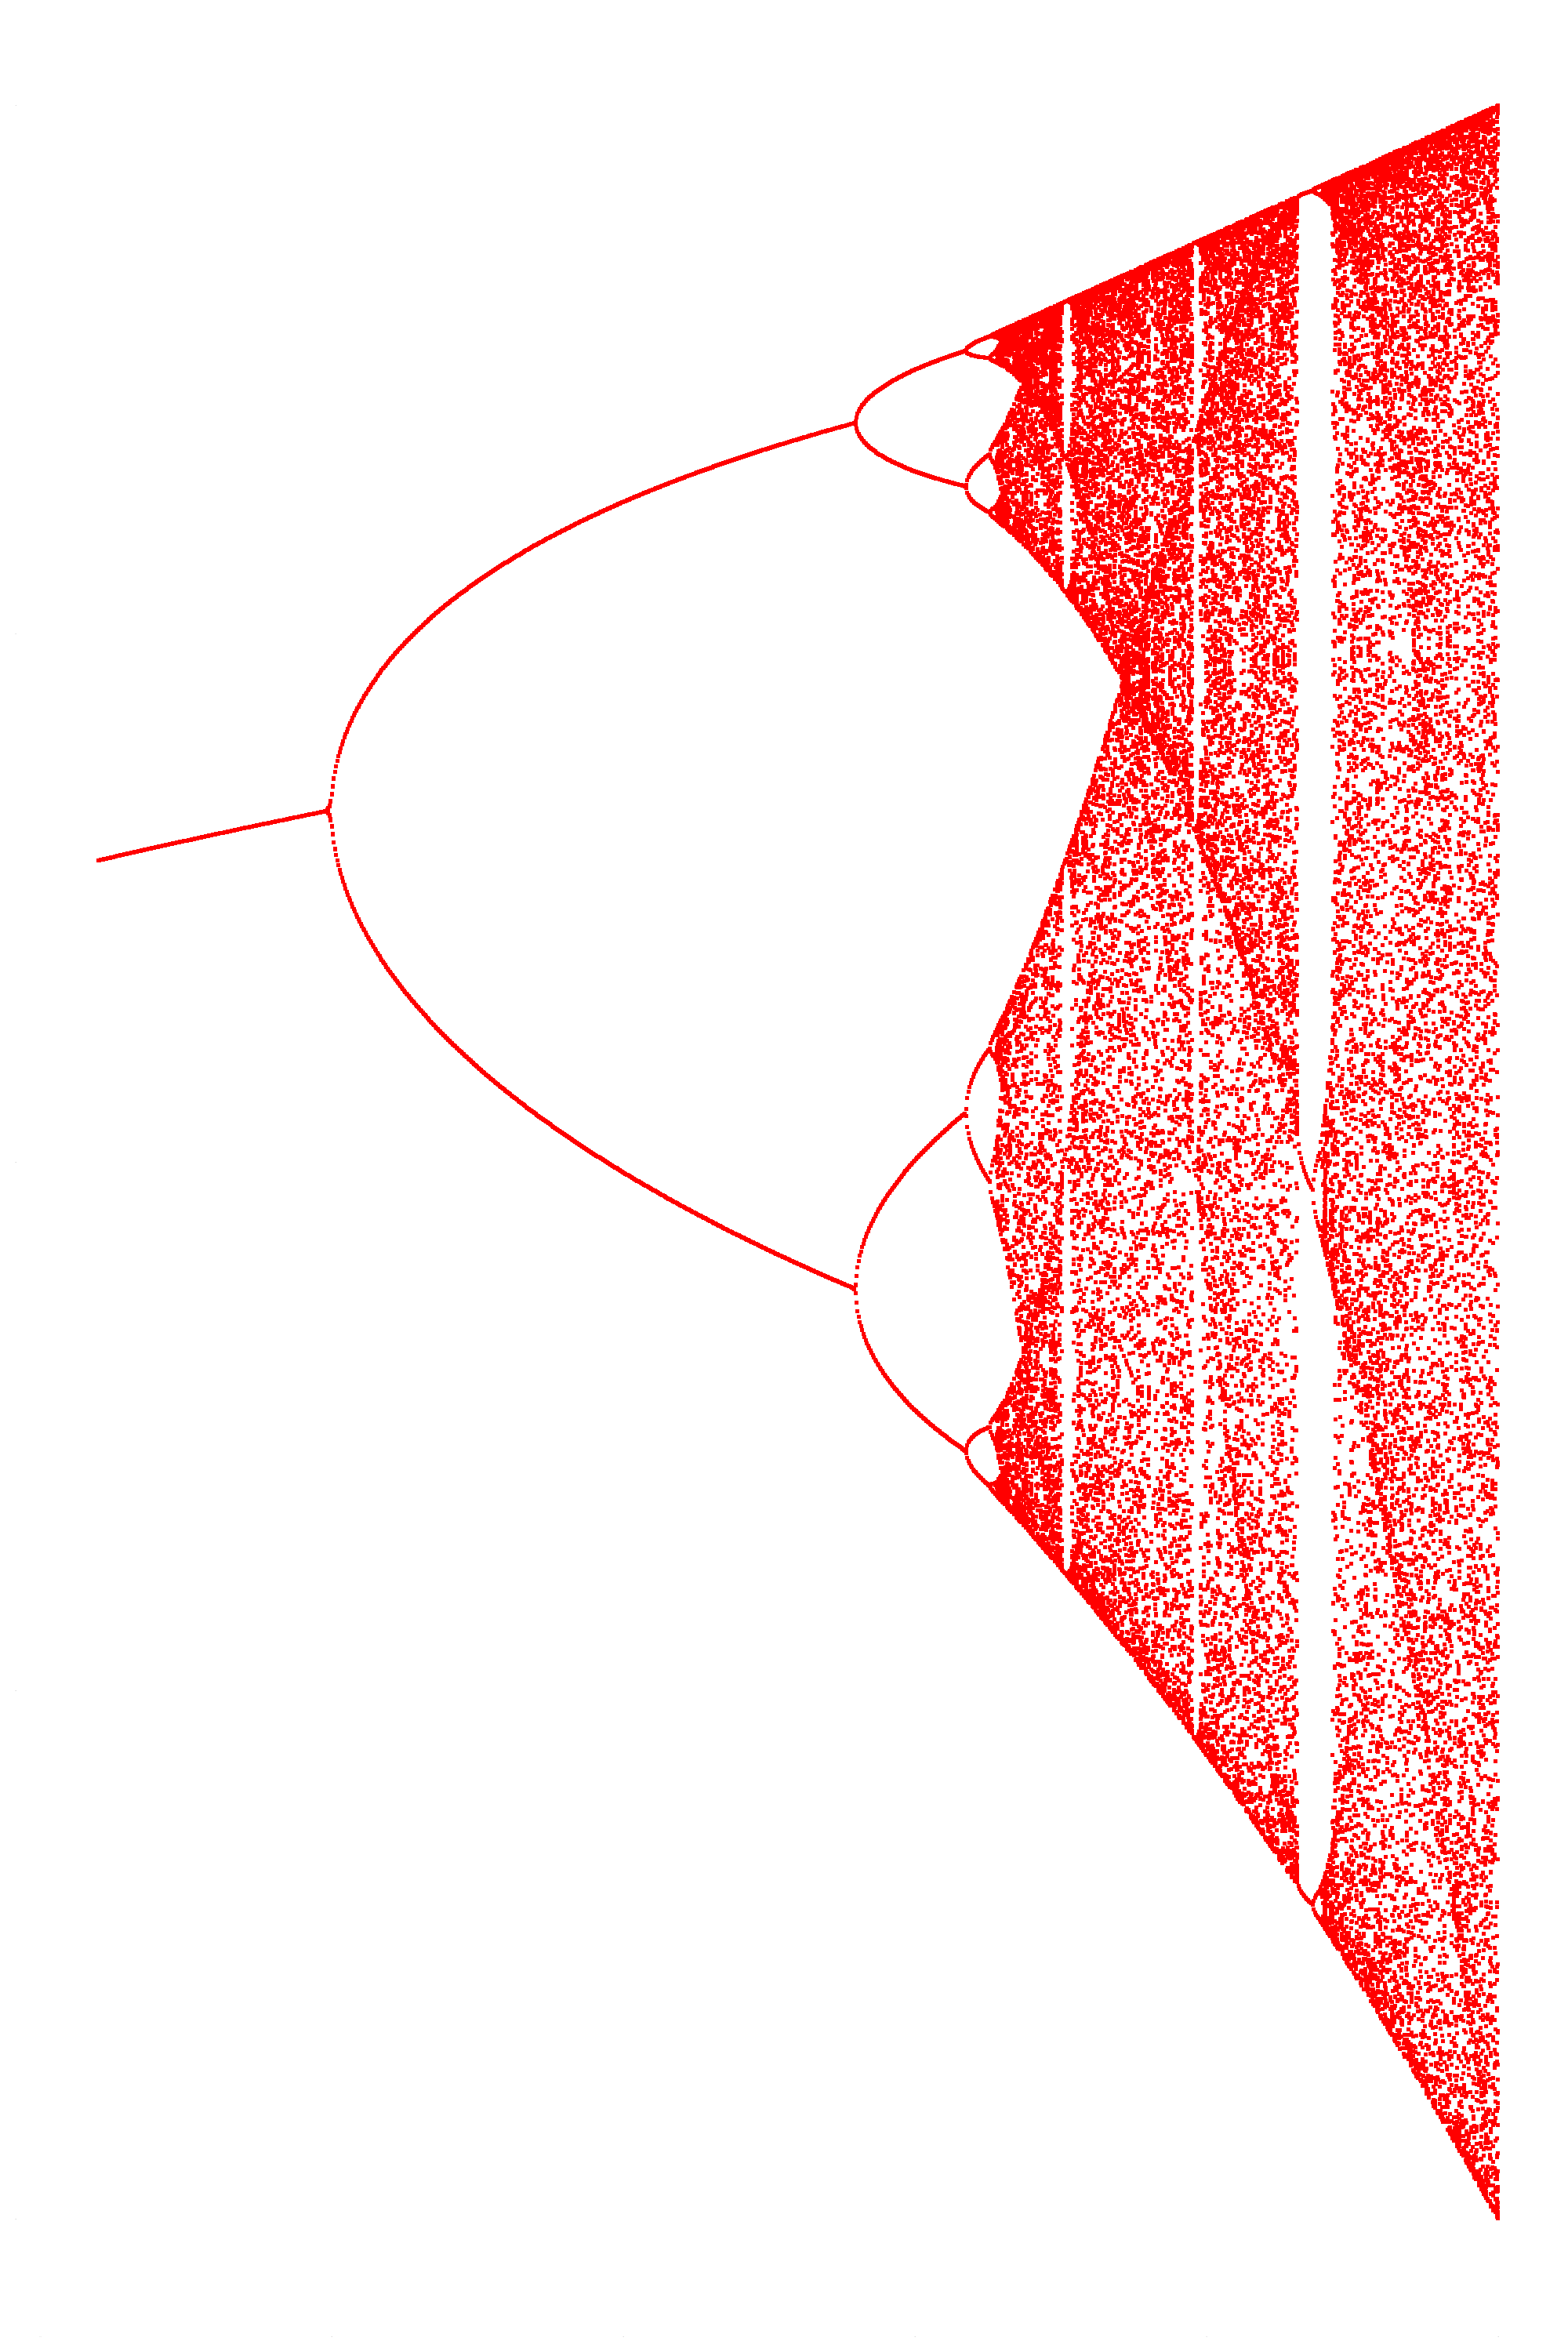
\includegraphics[width=0.75\textwidth]{figures/logistic_bifurcation.png}
			
		\end{center}
	\end{titlepage}
	\tableofcontents
	\part{Evolutionary Game theory and adaptive dynamics}
	\chapter{Evolutionary game theory for mathematicians}\label{background_EGT}
Nature is full of situations in which the fitness of organisms is frequency-dependent, in the sense that the `fitness payoff' to an individual adopting a `strategy' depends on the strategies adopted by other individuals in the population. Evolutionary game theory tries to capture the dynamics of such systems using a class of models called `evolutionary games'. Below, I will present (without proof) some notions and results from evolutionary game theory. Proofs of the results can be found in~\cite{broom_game-theoretical_2022} and sources cited therein.

\section{Games, strategies, and populations}
\definition{\emph{(Evolutionary Game)}}{ An $n$-player evolutionary evolutionary game is a collection $\{S_1,\cdots,S_n;g_1,\cdots,g_n\}$ of sets $S_i$ and functions $g_i:(S_1 \times S_2 \times \cdots \times S_n) \to \mathbb{R}$. $S_i$ is called the pure strategy set available to player $i$, and $g_i:(x_1,\cdots,x_n)\mapsto g_i(x_1,\cdots,x_n)$ is called the payoff function for player $i$ when player $j$ is playing strategy $x_j \in S_j$.}
Unless specified otherwise, we will assume that every player has access to the same set of pure strategies, in which case the evolutionary game can be characterized by the collection $(S,G)$, where $S$ is the pure strategy set and $G:(S\times S \times \cdots \times S) \to \mathbb{R}$ is the payoff function.
Thus, the game $(S,G)$ is modelling a situation in which every organism must choose some action from a set $S$, and the net benefit, or `payoff', of every action in $S$ is determined by the function $G$. We will in our discussion here restrict ourselves to the situation in which $S$ is finite\footnote{In general, $S$ need not be finite or even countable, it only needs to be measurable. In this setting, we must be careful with assigning payoffs and probabilities, and generally proceed by identifying a suitable $\sigma$-algebra $\mathcal{F}$ of $S$ over which to analyze the game (for example, if $S$ is also a topological space, the space of Borel sets of $S$ is usually a good choice). Then, each mixed strategy is a probability measure $\mu \in \mathbb{M}$ on $(S,\mathcal{F})$, payoffs are $\mu$-measurable real functions, and average payoffs are in terms of Lebesgue integrals over $(S,\mathcal{F},\mathbb{M})$. This more general setting is tricky to handle and is likely overkill for our sake, so we stick to cases where $S$ is a finite set and everything is `nice'.}. The finiteness of the pure strategy set is meant to model situations in which organisms have to `choose' between $m$ distinct, discrete alternatives.
If $S$ is a finite set $S = \{S_1,\cdots,S_m\}$, we say that the game is played on $m$ `pure' strategies. But what does this mean? What exactly does it mean to adopt a strategy?

\definition{\emph{(Strategy) }}{Given a game with pure strategy set $S = \{S_1,\cdots,S_m\}$, A \textit{strategy} is defined as a probability vector $p =  (p_1,\cdots,p_m)$ such that a player playing strategy $p$ plays $S_i \in S$ with probability $p_i$. A player playing strategy $p$ is called a $p$-player. Note that given a set of $m$ pure strategies, all strategies lie on the $m$-simplex $\Delta^{m}=\{(x_1,\cdots,x_m):x_i > 0, \sum\limits_{i=1}^{m} x_i = 1\}$}. This is sometimes called the strategy simplex.
\definition{\emph{(Support of a strategy)}}{ The \textit{support} of a strategy $p$ is the set of indices of non-zero elements of $p$, \textit{i.e} $\textrm{supp}(p) = \{i:p_i > 0\}$.}

\definition{\emph{(Pure and mixed strategies)}}{ Let $p \in \Delta^{m}$ be a strategy. If $|\textrm{supp}(p)| = 1$, we say that $p$ is a pure strategy, and otherwise, we say that $p$ is a mixed strategy. If $p$ uses every pure strategy (\textit{i.e} $p_i > 0 \ \forall \ i$, or $|\textrm{supp}(p)|=|S|=m$), we say that $p$ is an internal strategy, since it is in the interior of $\Delta^m$.}\\
\\
In biology, we are generally interested in a population of individuals, all of which are playing some game. Thus, we are interested in the payoff for an individual in a particular population. This idea is made precise below.

\definition{\emph{(Population)}}{ We will use $\delta_{p}$ to represent a population in which a randomly chosen player is almost surely a $p$-player. Note that we can write any population $\Pi$ as $\Pi = \sum\delta_{S_i}p_i$, where each $S_i$ is a pure strategy, and the probability of encountering an $S_i$-player is $p_i$. Unless otherwise specified, we will assume that populations are well-mixed and infinitely large.}\\
\\
We will use $\mathbb{E}[p;\Pi]$ to denote the expected payoff of a $p$-player in a population $\Pi$. When modeling dynamics, this is usually assumed to be equivalent (up to a constant) to the fitness of $p$-players in a population $\Pi$.\\
\\
The most well-known evolutionary games are matrix games, $i.e$ games for which one can define a (fixed) payoff matrix $A$ such that for any strategy $p$ in any population $\delta_q$, the expected payoff can be written as $\mathbb{E}[p;\delta_{q}]=qAp^T$. Note that this is equivalent to assuming that individuals are engaged in pairwise contests. Furthermore, note that $\mathbb{E}$ is linear in both $p$ and $q$. However, in many biologically relevant games, one cannot make this assumption. A more general class of evolutionary games are the so-called `playing-the-field' games, in which an organism is envisioned as playing against the population `as a whole'. This notion is made precise below.

\definition{\emph{(Playing the field)}}{ An evolutionary game is said to be a playing-the-field game if for any strategy $p=(p_1,\cdots,p_n)$ in any population $\Pi$, we can write
	\begin{equation*}
		\mathbb{E}[p;\Pi] = \sum\limits_{i=1}^{n}p_{i}f_i(\Pi)
	\end{equation*}
	where each $f_i:\Delta^{n}\to\mathbb{R}$ can be any (fixed) nonlinear function.
}\\
\\
Note that in playing-the-field games, $\mathbb{E}$ is linear in the focal player's strategy $p$, but need not be linear in the population strategy $q$. It is also clear that every matrix game with payoff matrix $A = (a_{ij})_{n\times n}$ is a playing-the-field game, with $f_i(q) = \sum\limits_{j=1}^{n}a_{ji}q_j = (A^Tq^T)_i$. Playing-the-field games are thus one of the two natural ways to try and generalize matrix games to model more varied biological phenomena\footnote{the other being to make payoffs linear in the population strategy but not the player strategy. My admittedly limited understanding is that this latter approach has found lesser applicability}

\section{Nash Equilibria, ESSs, and associated results}\label{subsection_NE_and_ESS}
I will now define two important notions which will characterize the types of strategies we are interested in.
\definition{\emph{(Nash Equilibrium)}}{ Consider a game on $n$ strategies. A strategy $p^{*}$ is said to be a \textit{Nash equilibrium} for the game if:
	\begin{equation*}
		\mathbb{E}[p^*;\delta_{p^*}] \geq \mathbb{E}[q;\delta_{p^*}] \ \forall \ q \neq p^* \in \Delta^{n}
	\end{equation*}
}\label{def_NE}
This definition is saying that if $p^*$ is a Nash equilibrium, then no $q$-player can do better than a $p^*$-player in a population of (almost surely) $p^*$-players, unless $q=p^*$. However, in evolutionary game theory, this is not a strong enough condition. We are generally interested in a stronger notion that allows for the possibility of small `invasions' of other `mutant' strategies that occur with \textit{non-zero} probability.
\definition{\emph{(ESS)}}{ Consider a game on $n$ strategies. A strategy $p^*$ is said to be an \textit{evolutionarily stable strategy (ESS)} for the game if $\forall \ q \neq p^* \in \Delta^{n} \ \exists \ \epsilon_q > 0$ such that:
	\begin{equation*}
		\mathbb{E}[p^*;(1-\epsilon)\delta_{p^*}+\epsilon\delta_q] >  \mathbb{E}[q;(1-\epsilon)\delta_{p^*}+\epsilon\delta_q] \ \forall \ \epsilon \in (0,\epsilon_q)
\end{equation*}}
Thus, if $p^*$ is an ESS, it is \textit{strictly} better than any other strategy $q$ when the population is comprised mostly of $p^*$-players, with some sufficiently small fraction $\epsilon$ of `mutant' $q$ players. Note that given any ESS $p^*$ and any strategy $q \neq p^*$, by taking the limit $\epsilon \to 0$ in the definition of an ESS, we see that $\mathbb{E}[p^*;\delta_{p^*}] \geq \mathbb{E}[q;\delta_{p^*}]$. Thus, if a strategy is an ESS, it must also be a Nash equilibrium.\\
Below, I will list some results pertaining to ESSs.
\begin{theorem}{\emph{(Characterization)}}\label{characterization}
	Let $h_{p,q,u}$ be the function\footnote{$h_{p,q,u}$ is often called the `incentive function', since it can be interpreted as the `incentive' of switching from strategy $q$ to strategy $p$ in a population where a fraction $u$ of the individuals are $q$-players and the rest are $p$-players.}:
	\begin{equation*}
		h_{p,q,u} = \mathbb{E}[p;(1-u)\delta_p+u\delta_q] - \mathbb{E}[q;(1-u)\delta_p+u\delta_q]
	\end{equation*}
	If $h_{p,q,u}$ is differentiable with respect to u at $u=0$ for every $p,q \in \Delta^{n}$, then $p$ is an ESS iff for every $q \neq p$, the following are true\footnote{condition 1 is often called the `equilibrium condition', and condition 2 is often called the `stability condition'. Maynard Smith, working only with matrix games, originally defined the notion of an ESS using these two criteria, with the stability condition as $\mathbb{E}[p;\delta_p]=\mathbb{E}[q;\delta_p] \Rightarrow \mathbb{E}[p;\delta_q]>\mathbb{E}[q;\delta_q]$. This characterization in terms of the incentive function shows that our definition in terms of $\epsilon$s generalizes his original definition.}:
	\begin{enumerate}
		\item $\mathbb{E}[p;\delta_p] \geq \mathbb{E}[q;\delta_p]$
		\item If $\mathbb{E}[p;\delta_p] = \mathbb{E}[q;\delta_p]$, then
		\begin{equation*}
			\frac{\partial h_{p,q,u}}{\partial u}\bigg{|}_{u=0} > 0
		\end{equation*}
	\end{enumerate}
\end{theorem}
%\begin{theorem}\emph{(Performance of pure strategies in the %support)}
%Consider a game in which $\mathbb{E}$ is linear in the focal player strategy and $h_{p,q,u}$ is differentiable at $0$ for every $p,q$. Let $p^*$ be an ESS. Then, $\mathbb{E}[S_i;\delta_{p^*}]=\mathbb{E}[p^*;\delta_{p^*}]$ for any $i \in \textrm{supp}(p^*)$.
%\end{theorem}
%In other words, any pure strategy that is in the support of an ESS performs just as well as the ESS itself in a population almost surely consisting of just the ESS.
How else can we identify ESSs? The following theorem examines
how an ESS behaves when playing against strategies that are `very close' to the ESS.
\begin{theorem}\emph{(Local superiority)}
	\label{local_superiority}
	Consider a playing-the-field game on $n$ strategies. $p$ is an ESS for this game iff $\exists \ \epsilon > 0$ s.t. 
	\begin{equation*}
		\mathbb{E}[p;\delta_q] > \mathbb{E}[q;\delta_q] \ \forall \ q \neq p \in B_{n}(p,\epsilon) \subseteq \Delta^{n}
	\end{equation*}
	where $B_{n}(p,\epsilon)$ is the $n$-dimensional ball with radius $\epsilon$ centered at $p$.
\end{theorem}
This theorem says that in the case of playing-the-field games, $p$ is an ESS if and only if it is `locally superior', in the sense that if one considers any strategy $q$ that is sufficiently similar to $p$, then $p$ performs (strictly) better than $q$ in a population of $q$-players.
Sometimes, finding several ESSs is much easier if you already know that a certain strategy must be an ESS. In the case of matrix games (\textit{i.e} games for which you can write down a constant payoff matrix), the following theorem is extremely useful:

\begin{theorem}\emph{(Bishop-Cannings theorem)}
	Consider a matrix game with pure strategies $S_1,\cdots,S_n$. Let $p$ be an ESS for this game. Let $T(p)$ be the set of indices of all pure strategies which have the same payoff against $p$ as $p$ has against itself, \textit{i.e} $T = \{i \ : \ \mathbb{E}[S_i,p]=\mathbb{E}[p,p]\}$. Then, if $q$ is any strategy such that $\textrm{supp}(q) \subseteq T(p)$, $q$ is not an ESS for the matrix game.
\end{theorem}

Thus, given a single ESS, the Bishop-Cannings theorem dictates that certain other strategies cannot also be ESSs. This greatly reduces the total number of possible ESSs in matrix games, and thus helps analyze such models. For example, an immediate and powerful corollary of the Bishop-Cannings theorem is the following:

\begin{corollary}\emph{(Uniqueness of the internal ESS)}
	If an internal strategy $p$ is an ESS for a matrix game, then it is the only ESS for that game.
\end{corollary}

Thus, in the case of matrix games, it is sufficient to find a \textit{single} internal ESS, since the Bishop-Cannings theorem will then ensure that this ESS is unique. 

\section{Replicator dynamics and the folk theorem}

Often, we are not interested in particular strategies, but are instead interested in predicting the fate of a given strategy in  a given population of individuals. For any game, if one assumes that the fitness of a strategy in a population is given by its expected payoff, then the population dynamics are given by the associated `replicator equation' on $\Delta^n$:
\begin{equation}
	\label{replicator}
	\dot{p_i} = p_i(\pi_i(\mathbf{p})-\bar{\pi}(\mathbf{p}))
\end{equation}
where $\mathbf{p(t)}=(p_1(t),\cdots,p_n(t)) \in \Delta^m$ is the strategy vector that we are tracking, $\pi_i(\mathbf{p}) = \mathbb{E}[S_i;\sum\limits_{i=1}^{n} p_i\delta_{S_i}]$ is the expected payoff of an $S_i$-player in a population where the probability of encountering an $S_i$-player is $p_i$, and $\bar{\pi}(\mathbf{p}) = \sum\limits_{i=1}^{n}p_i\pi_i(\mathbf{p})$ is the average payoff/fitness of the population.\\
Equation \eqref{replicator} defines a system of $n$ coupled ODEs, which has always has a unique solution\footnote{Assuming all functions are `nice': Specifically, we require that each $\pi_i$ is Lipschitz continuous in $\Delta^n$. In almost all practical cases, this will be satisfied.} given an initial condition $\mathbf{p}(0)=\mathbf{p}_{0}$. Biologically, we are interested in stable fixed points, \textit{i.e.} points $\mathbf{p^*}$ at which $\dot{p^{*}_i} = 0 \ \forall \ i$ and trajectories which are `close enough' to $\mathbf{p^*}$ converge to $\mathbf{p^*}$. If we were to find such points, then we could reason that populations which contain such a mix of individuals will maintain them forever, even in the face of small perturbations from the fixed point (due to, say, mutations or invasions from other populations). In the case of matrix games, the following theorems prove very useful and provide a connection between replicator dynamics and the notions introduced in section \ref{subsection_NE_and_ESS}:
\begin{theorem}\emph{(Folk theorem of evolutionary game theory) }
	If $p$ is an ESS for a matrix game, then $p$ is also a locally asympotically stable fixed point for the replicator dynamics associated with that game. Further, if $p^*$ is any fixed point for the replicator equations such that it is also the limit of at least one interior trajectory\footnote{\textit{i.e} $\exists \ p_0 \ \in int(\Delta^n) \ \textrm{s.t.} \ p(0) = p_0 \ \Rightarrow \lim\limits_{t\to\infty}p(t)=p^*$. Alternatively, it is also sufficient if the fixed point $p^*$ is instead Lyapunov stable}, then $p^*$ must be a Nash equilibrium for that game. In particular, every stable fixed point for the replicator dynamics is a Nash equilibrium for the game.
\end{theorem}
\begin{theorem}\emph{(Zeeman, 1980) }
	If $p$ is an internal ESS for a matrix game, then it is a global attractor for the associated replicator equation in $\textrm{int}(\Delta^n)$, \textit{i.e} every trajectory that starts within the interior of $\Delta^n$ converges to $p$.
\end{theorem}
Thus, in the case of matrix games, these theorems along with the Bishop-Cannings theorem tell us that identifying ESSs and Nash equilibria lets us characterize almost all the interesting properties of the game that we are interested in. This is why ESSs have played such a central role in evolutionary game theory. The first part of the Folk theorem (ESS $\Rightarrow$ stable fixed point) also holds for playing-the-field games (though the other results presented here do not). It is thus desirable to seek out ESSs even when trying to analyze a playing-the-field game.

\section{An example: The ideal free distribution as an evolutionary game}

The ideal free distribution was first formulated by Fretwell and Lucas in 1970 to study the distribution of birds in patchy environments. Fretwell and Lucas considered an environment with $n$ patches of unequal resources, where the $i$\textsuperscript{th} patch had resources of value $B_i$. Without loss of generality, we can renumber the patches such that $B_1 > B_2 > \cdots > B_n$. They further assumed that the value of the resource to each individual in the $i$\textsuperscript{th} patch was dependent on the interspecific competition on the $i$\textsuperscript{th} patch, which they modeled using a continuous increasing function $f_i(x_i)$, where $x_i$ is the density of individuals on the $i$\textsuperscript{th} patch, and $f_i(0) = 0$. Then, the net of the $i$\textsuperscript{th} patch when the $i$\textsuperscript{th} patch has a population density of $x_i$ is given by:
\begin{equation}
	\label{original_IFD}
	R_i(x_i) = B_i - f_i(x_i)
\end{equation}
They further assumed that individuals had complete knowledge of the value of every patch, that individuals were free to move from patch to patch with no cost, and that individuals moved between patches in order to maximize the net benefit $R_i$. Under these conditions, Fretwell and Lucas reasoned as follows: For any given organism in a given patch, if moving to any other patch would have been better for this individual, it would immediately do so. Thus, the only way to attain an `equilibrium' is if the organism \textit{cannot do any better} in any other patch than it is currently doing in the patch that it is on. Further, this should be true for every organism, and thus in every patch. This leads us to the conclusion that we require $R_1 = R_2 = \cdots = R_n$ if every patch is occupied. If only some number $l < n$ of patches are occupied at equilibrium, then these patches must be the ones with the $l$ greatest values of $B_i$, and we instead require $R_1 = R_2 = \cdots = R_l \geq B_{l+1} \geq B_{l+2} \geq \cdots \geq B_n$, since no patches past the $l$\textsuperscript{th} patch are occupied and patches are arranged in descending order of $B_i$. They dubbed such a distribution the `ideal free distribution' (IFD), and were able to study some properties of such a distribution.

\subsection{The game-theoretic perspective: A habitat selection game}
This idea of a scenario in which no organism can do better by moving to a different patch should immediately have you thinking of definition \ref{def_NE}. In fact, even though Fretwell and Lucas were unaware of this, it was quickly established that the IFD is likely a Nash Equilibrium for a cleverly defined game. In the early 2000s, Cressman, Krivan, and other game theorists defined the following `habitat selection game':
\definition{\emph{(Habitat selection game)} }{ Define a game on $n$ pure strategies where the $i$\textsuperscript{th} pure strategy $S_i$ is to stay on the $i$\textsuperscript{th} patch, and where the payoff of the $i$\textsuperscript{th} pure strategy in a population $(x_1,\cdots,x_n)$ given by $R_i = B_i - f_i(x_i)$. This game is called the `habitat selection game'.}
\\
In the habitat selection game, the expected payoff of a strategy $p$ in a population $\Pi=\sum q_i\delta_{S_i}$ is given by:
\begin{equation}
	\label{IFD_exp_payoff}
	\mathbb{E}[p;\Pi] = \sum\limits_{i=1}^{n}p_i(B_i-f_i(q_i))
\end{equation}
Note that this is linear in $p$ (but not necessarily linear in $\Pi$), and the habitat selection game is thus a playing-the-field game. In this new game-theoretic framework, we have the following definition:
\definition{\emph{(IFD strategy)} }{\label{def_IFD_strategy}A strategy $p$ for the habitat selection game on $n$ pure strategies is said to be an IFD strategy if there exists $l \leq n$ such that:
	\begin{enumerate}
		\item $p_i > 0 \iff i \leq l$
		\item $R_1 = R_2 = \cdots = R_l \geq B_{l+1} \geq \cdots \geq B_n$
\end{enumerate}}
This puts the IFD that Fretwell and Lucas recognized in game-theoretic terms. Though the game-theoretic aspect of the original IFD as proposed by Fretwell and Lucas was implicitly recognized for a long time, it was only in 2006 that the habitat selection game was defined, and it was proved both that the IFD is in fact an ESS for the habitat selection game, and that \textit{any} ESS for the habitat selection game must be an IFD strategy. We state and prove this as a theorem below.
\begin{theorem}\emph{(Cressman \textit{et al.}, 2006)}\label{theorem_original_IFD}
	A strategy $p$ is an ESS for the habitat selection game iff it is an IFD strategy.
\end{theorem}
\begin{proof}
	Assume that $p= (p_i)_i$ is an ESS for the habitat selection game. We will prove that it is an IFD, \textit{i.e} that it satisfies both criteria listed in  definition \ref{def_IFD_strategy}.\\
	To see that it satisfies the first criterion, assume the contrary, \textit{i.e.} that there exist $j < k \leq n$ such that $p_j = 0$ and $p_k > 0$. Then, 
	
	\begin{equation}
		\label{ESS_to_IFD_1}
		R_j = B_j - 0 = B_j \geq B_k > B_k - f_k(p_k) = R_k
	\end{equation}
	Define $\Tilde{p}$ as:
	\begin{equation*}
		\Tilde{p}_i = \begin{cases}
			p_i & i \neq j,k \\
			p_k & i = j\\
			p_j & i = k
		\end{cases}
	\end{equation*}
	Thus, $p_l = \Tilde{p}_l$ everywhere except at $j$ and $k$, where the values are switched. The incentive function $h_{p,\Tilde{p},0}$ is given by:
	\begin{equation*}
		h_{p,\Tilde{p},0} = \mathbb{E}[p;\delta_p] - \mathbb{E}[\Tilde{p};\delta_p]
	\end{equation*}
	Using equation \eqref{IFD_exp_payoff}, we get:
	\begin{align*}
		h_{p,\Tilde{p},0} &= \sum\limits_{i=1}^{n}(p_i-\Tilde{p}_i)(R_i)\\
		&= -\Tilde{p}_jR_j + p_kR_k\\
	\end{align*}
	But since $\Tilde{p}_j = p_k$, using equation \eqref{ESS_to_IFD_1}, we get:
	\begin{equation*}
		h_{p,\Tilde{p},0} = p_k(R_k-R_j) < 0
	\end{equation*}
	which contradicts the necessary part of theorem \ref{characterization}, thus yielding a contradiction. If payoffs of the occupied patches are unequal, \textit{i.e} if there exist $j,k \leq l$ such that $R_j > R_k$, we can similarly define
	\begin{equation*}
		\Tilde{p}_i = \begin{cases}
			p_i & i \neq j,k \\
			p_j + p_k & i = j\\
			0 & i = k
		\end{cases}
	\end{equation*}
	to yield the same contradiction, by following the same steps. Lastly, if $l$ patches are occupied in the population and there are $j \leq l < k$ with $R_l < B_k$, we can define
	\begin{equation*}
		\Tilde{p}_i = \begin{cases}
			p_i & i \neq j,k \\
			p_k & i = j\\
			p_j & i = k
		\end{cases}
	\end{equation*}
	to arrive at a contradiction through the same steps, leading us to the conclusion that $R_1 = \cdots = R_l \geq B_{l+1} \cdots B_n$. We have thus proved that every ESS is an IFD strategy. We will now prove the converse.\\
	\\
	Assume that $p=(p_i)_i$ is an IFD strategy with $l$ patches occupied. We will use the local superiority property to prove that $p$ is an ESS. Consider any strategy $q \neq p$.
	\\
	\\
	\begin{mycase}
		\case All patches are occupied in the IFD (\textit{i.e} $l = n$)
		\begin{quote}
			Let $R_1=\cdots=R_n=R^*$. We have:
			\begin{align}
				\sum\limits_{i=1}^{n}(p_i-q_i)(B_i-f_i(p_i)) &= \sum\limits_{i=1}^{n}(p_i-q_i)R_i(p)\\
				&= R^*\sum\limits_{i=1}^{n}(p_i-q_i)\nonumber\\
				&= R^*(\sum\limits_{i=1}^{n}p_i-\sum\limits_{i=1}^{n}q_i)\nonumber\\
				&= R^*(1-1) = 0\label{IFD_to_ESS_zero_sum}
			\end{align}
			Now, consider the quantity $\mathbb{E}[p;\delta_q]-\mathbb{E}[q;\delta_q]$. Subtracting the LHS of \eqref{IFD_to_ESS_zero_sum} from this, we have:
			\begin{align}
				\mathbb{E}[p;\delta_q]-\mathbb{E}[q;\delta_q] &= \sum\limits_{i=1}^{n}(p_i-q_i)(B_i-f_i(q_i))\nonumber\\
				&= \sum\limits_{i=1}^{n}(p_i-q_i)(B_i-f_i(q_i))- \sum\limits_{i=1}^{n}(p_i-q_i)(B_i-f_i(p_i))\nonumber\\
				&= \sum\limits_{i=1}^{n}(p_i-q_i)(f_i(p_i)-f_i(q_i))\label{IFD_to_ESS_local_sup}
			\end{align}
			By definition, each $f_i$ is assumed to be a strictly increasing function. It is easy to see that this implies that $(p_i-q_i)(f_i(p_i)-f_i(q_i))>0 \ \forall \ i$. Using this in \eqref{IFD_to_ESS_local_sup}, we see that $\mathbb{E}[p;\delta_q]-\mathbb{E}[q;\delta_q] > 0 \ \forall \ q \neq p$. Thus, $p$ is locally superior, and by the necessary part of theorem \ref{local_superiority}, it must be an ESS.
		\end{quote}
		\case Some patches are unoccupied in the IFD (\textit{i.e} $l<n$)
		\\
		\begin{quote}
			Let $R_1=\cdots=R_l=R^*$. As before, we examine the quantity:
			\begin{align}
				\sum\limits_{i=1}^{n}(p_i-q_i)(B_i-f_i(p_i)) &= \sum\limits_{i=1}^{l}(p_i-q_i)(B_i-f_i(p_i)) + \sum\limits_{i=l+1}^{n}(p_i-q_i)(B_i-f_i(p_i))\nonumber\\
				&= \sum\limits_{i=1}^{l}(p_i-q_i)R^* - \sum\limits_{i=l+1}^{n}q_iB_i\label{IFD_to_ESS_case_2_ineq_1}
			\end{align}
			Where the last equality comes from the definition of an IFD strategy on $l$ patches as having $p_i > 0 \iff i \leq l$ and the definition of each $f_i$ as satisfying $f_i(0)=0$. Using the fact that $R^* \geq B_k \ \forall k > l$ in \ref{IFD_to_ESS_case_2_ineq_1}, we now get:
			\begin{align*}
				\sum\limits_{i=1}^{n}(p_i-q_i)(B_i-f_i(p_i)) &\geq \sum\limits_{i=1}^{l}(p_i-q_i)R^* - \sum\limits_{i=l+1}^{n}q_iR^*\\
				&= R^*(\sum\limits_{i=1}^{n}p_i - \sum\limits_{i=1}^{n}q_i)\\
				&= R^*(1-1) = 0
			\end{align*}
			We can now proceed as in case 1 and write
			\begin{align*}
				\mathbb{E}[p;\delta_q]-\mathbb{E}[q;\delta_q] &= \sum\limits_{i=1}^{n}(p_i-q_i)(B_i-f_i(q_i))\\
				&> \sum\limits_{i=1}^{n}(p_i-q_i)(B_i-f_i(q_i))- \sum\limits_{i=1}^{n}(p_i-q_i)(B_i-f_i(p_i))\\
				&= \sum\limits_{i=1}^{n}(p_i-q_i)(f_i(p_i)-f_i(q_i)) \\
				&\geq 0 \ \forall \ q \neq p \ \ (\because \textrm{every $f_i$ is increasing)}
			\end{align*}
			and thus, $p$ is locally superior and therefore an ESS by theorem \ref{local_superiority}. This concludes our proof.
		\end{quote}
	\end{mycase}
\end{proof}
Thus, for the habitat selection game as defined above, every ESS is an IFD strategy, and every IFD strategy is an ESS. It is also possible to prove that for the game defined above, there is a single unique ESS (and thus IFD). The habitat selection game and the IFD concept have been extended in various directions, such as to include multiple species (each with a different $B_i$ and $f_i$ set), migration dynamics, costs to migration, and incomplete information. 
	

\chapter{Adaptive Dynamics}

\textbf{Note: This chapter is taken almost verbatim from Gaurav Athreya's Master's thesis~\citep{athreya_thesis_2023}, with permission. I (Shikhara) have made some minor edits to make it fit in with the rest of the Napkin.}
\\

{\color{red}TODO: add general intro text here}

In an unstructured population (no life-stages, no spatial structure, etc.) the use-cases of this framework may be built up in complexity as follows
\begin{itemize} \itemsep -1mm
	\item one type with one evolving trait
	\item one type with several evolving traits
	\item several interacting types each with one evolving trait each
	\item several interacting types with several evolving traits each
\end{itemize}  

In each case, two things must be clear to the reader by the end of this document: how to actually compute invasion fitness, and then how to analyse the evolutionary dynamics induced by an invasion fitness function. 

\section{Adaptive dynamics for a one-dimensional trait}
\label{section:1-dim-AD}

Consider a trait taking values in $T \subset \mathbb{R}$ and an asexual population monomorphic for this trait. We define the \emph{fitness} of a strategy as its long-term exponential growth rate in a given environment. 
In particular, suppose $r(x, E_x)$ denotes the fitness of a phenotype $x$ in an environment $E_x$ consisting of constant abiotic factors and other $x$ individuals.
When $x$ is a demographic attractor (e.g. a fixed point), $r(x, E_x) = 0$ since the population abundances do not change and hence the growth rate is zero. 
Now consider a rare mutant phenotype $y$ that arises in a background resident population having equilibrium phenotype $x$.  
As long as the mutant is rare, it does not have an appreciable effect on the environment and its fitness is hence $r(y, E_x)$. 
For convenience we shall denote this quantity by $f(x,y)$, and call it the \textit{invasion fitness} of mutant $y$ in a resident population of $x$. 
We assume that this function is sufficiently smooth in both coordinates. 

\subsection{Analytic classification of singular points}

If $f(x,y)>0$, the mutant can spread but might go to extinction due to small-size stochastic extinction. 
If $f(x,y)<0$, it will die out. 
If $f(x,y)>0$ and $f(y,x)<0$, then the mutant can spread but the resident cannot recover when rare itself. 
In fact, it has been shown that it is usually enough that $f(x,y)>0$ for the mutant $y$ to invade \textit{and} fix -- sometimes called ``invasion implies substitution".  
Therefore, it is sufficient to just check when $f(x,y)>0$.
For complicated functional forms, the evolutionary dynamics is determined by the derivative of $f(x,y)$, also known as the \textit{fitness gradient}. 
This is because to first order, the fitness can be expressed as 
\begin{align}
	f(x,y) = \left. \frac{\partial f}{\partial y} \right|_{y=x} (y-x)
\end{align}
where $f(x,x) = 0$ by assumption. 
So the population evolves i.e., trait changes until it reaches a point where the fitness gradient is zero. 
Recall that the trait value of the population is changing by invasion of mutants which have positive invasion fitness. 
Such points are called evolutionarily singular points. 
We will now consider what happens when the population gets to (if it can) a singular point. 
One of the major virtues of the adaptive dynamics framework is that it differentiates explicitly between two different kinds of stability: evolutionary stability and convergence stability. 
As we will see, these are mutually exclusive and can occur in any combination. 

\begin{definition}
	A singular point $x^*$ is said to be locally evolutionarily stable if it cannot be invaded by any nearby strategy i.e., $f(x,y)<0$ for all $y$ in some neighbourhood around $x$. 
\end{definition}
Local evolutionarily stable points are traps in the sense that a population cannot escape from such a point via small mutations. 
It is easy to see that this is equivalent to the condition that the trait value $x^*$ is a (local) maximum for the function $f(x,y)$ in the mutant, $y$ direction. 
Evolutionary stable singular points are therefore characterized by 
\begin{align}
	\left. \frac{\partial^2 f}{\partial y^2} \right|_{y=x^*} < 0
\end{align}
Now for notational convenience, let us define 
\[
D(x) = \left. \frac{\partial f}{\partial y} \right|_{y=x}
\]
\begin{definition}
	A singular point $x^*$ is said to be \textit{convergence stable} if a population can reach the neighbourhood of $x^*$ i.e., (monomorphic) populations closer to the singular point can replace those farther away. 
	More formally, for any point $x<x^*$ in a neighbourhood around $x^*, f(x,y)>0 \ \forall y \in (x,x^*)$ and similarly, for any $x>x^*$ in a neighbourhood around $x^*, f(x,y)>0 \ \forall y \in (x^*,x)$. 
\end{definition}
In other words, the fitness gradient points toward the singular point. Since the fitness gradient must change sign from positive to negative, $D(x)$ must be a decreasing function and so at a convergence stable singular point, we must have 
\begin{align}
	\left. \frac{d}{dx} D(x) \right|_{x=x^*} < 0 
\end{align} 
Note that there is a relation between the conditions for convergence and evolutionary stability
\begin{align}
	\frac{dD(x)}{dx} = \frac{\partial^2 f}{\partial x \partial y} + \frac{\partial^2 f}{\partial y^2}
	\label{eqn: selection-gradient-1D}
\end{align}
where one can see that convergence stability requires the evaluation of the additional term on the left. 
Note here the important role of the assumption that mutations are not infinitesimal - if one were to assume that, a population would never actually reach a convergence stable point.

Thus, we arrive at the following classification of evolutionary singularities:
\begin{center}
	\begin{tabularx}{0.4\textwidth}{ 
			| >{\centering\arraybackslash}X 
			| >{\centering\arraybackslash}X 
			| >{\centering\arraybackslash}X | }
		\hline
		& \textbf{ES} & \textbf{not ES} \\
		\hline
		\textbf{CS} &  \circled{A}  &  \circled{B} \\ 
		\hline
		\textbf{not CS} & \circled{C}  & \circled{D} \\
		\hline
	\end{tabularx}
\end{center}

Points which are not convergent stable are not of interest to us because populations can only attain such a state if they begin there. Thus, \circled{C} and \circled{D} can be ignored for our purposes.\footnote{Singularities of type \circled{C} are sometimes called `garden of Eden' points, since a population that begins at such a point will remain there and cannot be invaded by nearby mutants, but if a population does not begin there (or is somehow driven out by external forces), it can never find its way back to the singularity.}\\
Points of type \circled{A} are both evolutionarily stable and convergent stable. Such points represent `endpoints' for evolution, since populations are attracted to such points and also cannot evolve away from them since they cannot be invaded by any nearby mutants.

An interesting case is to consider singular points which are convergence stable, but not evolutionarily stable ( type \circled{B} in our table). 
What happens at such points? 
The population can reach the point, but then it is susceptible to invasion by nearby mutants. Furthermore, it is susceptible to invasion from distinct types of mutants. To see this, let $x^*$ be such a point, and let $x_1 < x^* < x_2$ be two points in the immediate vicinity of $x^*$.
\begin{claim}
	Each of $x_1$ and $x_2$ can invade the other
\end{claim}
\begin{proof}
	Let $g(x) = dx/dt$ denote the fitness gradient for convenience.
	We can Taylor expand the invasion fitness function as
	\begin{align*}
		f(x_2 ,x_1) &= \underbrace{f(x_2 , x_2)}_{=0} + \underbrace{(x_1 - x_2)}_{< 0 }\underbrace{\frac{\partial f}{\partial x_1}(x_2, x_1)\bigg{|}_{x_1 = x_2}}_{=g(x_2)} + \frac{(x_1-x_2)^2}{2} \frac{\partial^2 f}{\partial x_1^2}(x_2 , x_1)\bigg{|}_{x_1 = x_2}
	\end{align*}
	where we have neglected terms that are higher than second order. Since $x^*$ is a singular point, $g(x^*) = 0$. Since $x^*$ is convergent stable, $\frac{d g}{dx}\bigg{|}_{x=x^*} < 0$ and we therefore see that $g$ is a decreasing function of $x$ in the immediate vicinity of $x^*$. Thus, since $x_2 > x^*$, we must have $g(x_2) < g(x^*) = 0$, and we can conclude that the second term in the RHS must be positive. Lastly, since $x^*$ is evolutionarily unstable, we must have $\frac{\partial^2 f}{\partial x_1^2}(x^*,x_1)\bigg{|}_{x_1 = x^*} > 0$ by the stability criterion. Thus, assuming $f$ is smooth, for $x_2$ sufficiently close to $x^*$, it must be the case that $\frac{\partial^2 f}{\partial x_1^2}(x_2,x_1)\bigg{|}_{x_1 = x_2} > 0$. Thus, the third term of the RHS is also positive, meaning that $f(x_2, x_1) > 0$, and that $x_1$ can thus invade $x_2$. An exactly analogous argument shows that $f(x_1,x_2) > 0$, thus completing the proof.
\end{proof}
This observation leads to the following definition:
\begin{definition}
	A \textit{protected polymorphism} is a polymorphic population in which none of the phenotypes can go extinct i.e., all have positive fitnesses when rare and therefore cannot be lost, and therefore none of them can fix. 
\end{definition}

After a small perturbation of a population of this type that is inevitable over the course of evolutionary time, we will have a resident that is slightly off the singular point, and a mutant that arises that is also off the singular strategy and has positive growth rate when rare. 
This necessarily gives rise to a protected dimorphism since both populations can recover when rare. 
We can show (see appendix 1 in \cite{geritz_evolutionarily_1998})  that such a population can be invaded only by mutants that are farther away from the singular strategy than the current population.
This gives rise to a diverging population with two ``branches" that progressively become more separated from each other with time. 
Such points i.e., those that are not evolutionarily stable but convergence stable, are known as branching points, and this phenomenon is termed \textit{evolutionary branching}.
Trait divergence takes place until another singular point is reached, or until the local approximations used in the above characterizations no longer hold. 

\subsection{Pairwise Invasibility Plots (PIPs) and graphical characterizations of singular points}

The evolution of a population can be studied also by means of a pairwise invasibility plot, which is a two-dimensional plot of the sign of $f(x,y)$ as a function of $x$ and $y$. 
In particular, the character of a singular point can be determined by the structure of `-' and `+' regions around it. 
The graphical characterization of the above properties is as follows:
\begin{enumerate}
	\item A \textbf{singular point} can be identified on the PIP since it will be in the intersection between the zero-set of $f(x,y)$ and the line $y=x$ (since $f(x,x)=0 \ \forall \ x$). 
	\item A singular point is \textbf{evolutionarily stable} if no mutant can invade it. Hence, the vertical line through it must be locally entirely within a `-' region. 
	\item For characterizing convergence stable points, we will make use of the diagonal $y=x$. A singular point $x^*$ is \textbf{convergence stable} if
	\begin{itemize}
		\item to the left of $x^*$, the area above $y=x$ is locally inside a `+' region
		\item to the right of $x^*$, the area below $y=x$ is locally inside a `+' region 
	\end{itemize}   
	\item \textbf{Continuously stable}: convergence stable and ESS, so (1), (2), (3)
	\item \textbf{Branching point}: convergence stable and not ESS, so conditions (1), (3) and negation (2)
\end{enumerate}

{\color{red}TODO: Maybe draw this?}

The difference between these two notions of stability is now clear: convergence stability describes whether an evolving population can actually reach the singular point, whereas evolutionary stability describes the invadability of a population already at the point. From both the algebraic and the graphical characterizations, one can see that neither condition implies the other - a singular point can be any combination of convergence stable (or not) and evolutionarily stable (or not).  

\subsection{An example of a prediction of adaptive dynamics}

Let us consider the invasion fitness function:
\begin{equation}
	\label{AD_cts_logistic_invasion_fitness}
	f(x,y) = 1 - \frac{\alpha(x,y)K(x)}{K(y)}
\end{equation}
This is a model of asexual resource competition:  $\alpha(x,y)$ is called the \emph{competition kernel} and $K(x)$ is called the \emph{carrying capacity function} (formulated in analogy with Lotka-Volterra competition or the logistic equation).  Let us ssume that we have $\alpha(u,v) = \exp{-(u-v)^2/(2\sigma^{2}_{\alpha})}$ and $K(u) = K_{0}\exp{-(u)^2/(2\sigma^{2}_{K})}$, \emph{i.e.} Gaussian carrying capacity and Gaussian competition kernel. Biologically, this means that phenotypes that are closer to each other compete more (through $\alpha$) and that there is also a single phenotype, $x=0$, that is optimal for the abiotic environment (through $K$). Then, it is easy to derive using the definitions of evolutionary stability and convergence stability that the population remains monomorphic if and only if
\begin{equation}\label{AD_monomorphic_condn}
	\sigma_K<\sigma_{\alpha}
\end{equation}
and evolves polymorphism otherwise.
\subsubsection{Habitat Filtering}
One way that \ref{AD_monomorphic_condn} can be satisfied is if $\sigma_K$ is very small. Biologically, this means that the environment is such that only some very particular morphs are viable, and the limit where $\sigma_K = 0$ corresponds to a case where only a single morph is environmentally viable. Ecologists are well-acquainted with this notion, and refer to it as `habitat filtering', the phenomenon in which the habitat itself `selects' for certain phenotypes due to particular limiting abiotic factors.

\subsubsection{Competition and character displacement}
A second way to satisfy \ref{AD_monomorphic_condn} is if $\sigma_{\alpha}$ is very large. Biologically, this means that competition occurs across a wide range of phenotypes, and the limit where $\sigma_{\alpha} = \infty$ corresponds to frequency-independent competition. In other words, diversification can fail if competition cannot be alleviated through character displacement, \emph{i.e} selection is not disruptive (or has a very weak disruptive component). This could happen if, for example, the morphs are competing for a resource that has no alternatives and can only be acquired in a single way (Ex: Competition for sunlight in plants).

\section{Microscopic descriptions and a stochastic derivation of the canonical equation of adaptive dynamics}
\label{section:microscopic-descriptions-CE}

The canonical equation of adaptive dynamics (CE) is a dynamical system that describes the evolution of phenotypic traits in terms of the fitness gradient and the mutational processes that give rise to variation.
\cite{dieckmann_dynamical_1996} showed that this (until then often heuristically invoked) equation has a solid foundation based in the microscopic interactions between individuals in the population.
Specifically, the CE describes the mean trajectory of a directed random walk in the trait space, with birth and death rates determined by the ecological processes operating in the population. 
In this section, we describe the underlying stochastic process, and derive the CE using the master equation for this stochastic process along with certain smoothness assumptions. 

Evolutionary dynamics takes place over long timescales, where we make all the simplifying assumptions stated above. 
Over shorter timescales, population dynamics is decided by ecological processes.
The fate of a mutant is thus determined by the ecology of its interaction with the resident. 
This is the link between the fitness of the previous section and mechanistic models of population dynamics - it is given by the growth rate of the mutant over ecological timescales. 

Consider a population consisting of $N$ types of individuals, with their abundances given by $n = (n_1, ..., n_N)$. 
Now consider a collection of traits $s = (s_1, ..., s_N)$ such that $s_i$ determines the birth and death rates of type $i$. 
These traits may be, for example, related to beak morphology in a population of interacting finches.
Due to the assumption that the ecological and evolutionary timescales are separated, this trait can be assumed to be constant for the ecological dynamics.  Then a general model of the population dynamics is given by 
\begin{align}
	\frac{dn_i}{dt} = (b_i(n) - d_i(n))  n_i \hspace{10mm} i = 1, ... , N
	\label{eqn:bi-di-eqn-form}
\end{align} 
where $n$ is the vector of type abundances and $b_i$ and $d_i$ are the birth and death rates of each type. 
We say the combined quantity $b_i-d_i$ is the \textit{growth rate}. 
Note that we have explicitly allowed the birth and death rates to be frequency dependent.

There is a corresponding stochastic process for the evolution of the traits $s$ that can be constructed given any model for short-timescale population dynamics of the above form. 
This is a continuous-time random walk on the state space $\mathcal{S}$ given by the Cartesian product of the state space of each $s_i$. 
Stochasticity in the trait value is due to mutation of the trait, and demographic stochasticity - small mutant populations may die out purely due to size. 
We assume that selection pressures only depend on this trait; it is always true that they depend only on the present value of a trait.
Mutation also depends only on the present value. 
The process can therefore be assumed to be Markovian, simplifying the analysis.

The time-evolution of the probability distribution is described by the master equation
\begin{align}
	\frac{d}{dt}P(s,t) = \int_ \mathcal{S} [P(s',t)w(s|s') - P(s,t)w(s'|s)] ds'
\end{align}
which basically measures flux into and out of the trait value $s$. 
The transition function $w(s_1|s_2)$ is determined by the composition and ecology of the population. 
Now, we give an expression for the transition function in terms of the transitions in each trait: we assume that no two species can simultaneously undergo a trait substitution in the infinitesimal time $dt$. 
Therefore, we can write
\begin{align}
	w(s'|s) = \sum_{i=1}^N w_i(s_i'|s) \prod_{j \ne i} \delta(s_j'-s_j)
\end{align}
In other words, add - for each $i$ - the probability of $s_i$ transitioning to $s_i'$ when all the other traits stay unchanged i.e.,  $s_j' (j \ne i)$ are still equal to $s_j$.
Next, we must derive an expression for the single trait transition functions $w_i(s'|s)$.
For this, we assume that mutation and selection are independent, so the probability per unit time $w_i$ for a specific trait substitution is given by the probability per unit time $\mathfrak{M}_i$ that the mutant is generated by an individual of the population times the probability $\mathfrak{S}_i$ that it successfully escapes size-related stochastic extinction. 
\begin{align}
	w(s_i'|s) = \mathfrak{S}_i (s_i',s) \mathfrak{M}_i (s_i',s)
\end{align}
We can then write expressions for the probabilities above in terms of previously defined quantities like the birth and death rates, equilibrium population size, and mutation distribution~\citep{dieckmann_dynamical_1996}.

Now define the average path
\begin{align}
	\left< s\right>(t) = \int_{\mathcal{S}} sP(s,t)ds 
\end{align}
Using the master equation, the Fubini-Tonelli theorem, and the Leibniz rule, we can write
\begin{align}
	\frac{d}{dt} \left< s \right> = \int \int (s'-s)w(s'|s) P(s,t)ds'ds
\end{align}
We now introduce the $k$th jump moment $a_k = (a_{k1},...,a_{kN})$ with 
\begin{align}
	a_{ki} = \int (s_i'-s_i)^k w(s_i'|s_i)ds_i'
\end{align}
Then we can write 
\begin{align}
	\frac{d}{dt}\left< s \right> = \left< a_1(s) \right>(t)
\end{align}
We linearize the first jump moment i.e., assuming it is twice differentiable, take only the linear term in the Taylor series and ignore the higher order terms. 
WLOG calling the linear part by the same name, we can say 
\begin{align}
	\frac{d}{dt}\left< s \right> =  a_1(\left< s \right>)(t)
\end{align}
Now we call the mean path variable by a different name $x$ for convenience. Substituting the exact expressions for $\mathfrak{S}_i$  and $\mathfrak{M}_i$ and Taylor-expanding the fitness term to first degree, we get
\begin{align}
	\frac{dx_i}{dt} = \frac{1}{2} \mu_i(x_i) \sigma^2_i(x_i) \hat{n}_i(x) \frac{\partial \bar{f}_i}{\partial x_i'} \hspace{10mm} i=1,....,N
\end{align}
where $\mu_i(x_i)$ is the fraction of births in the population that give rise to mutations in type $i$, $\sigma^2_i(x_i)$ is the variance of the mutation distribution, $ \hat{n}_i(x)$ is the equilibrium population at the trait value $x$, $\bar{f}_i$ is the time-averaged growth rate, which is equal to $f(s, \hat{n}(s))$. 
This is the canonical equation of adaptive dynamics. 
This shows that the right notion of fitness for the mutant is its average growth rate $\bar{f}_i = \left. b_i(n)-d_i(n) \right|_{n=n^*} $ when rare in a resident population at equilibrium.
If the traits under considering for each type number more than one each, some changes need to be made to the above equation. 
Let the fitness of type $i$ now be determined by $v_i$ traits. 
Firstly, $\sigma^2_i(x_i)$ now becomes the variance-covariance matrix of the mutation distribution. 
Secondly, the fitness gradient  $\frac{\partial \bar{f}_i}{\partial x_i'}$ now becomes the multidimensional gradient $\nabla_i'f(x_i',x)$.  Therefore, the multi-dimensional CE is given by
\begin{align}
	\frac{dx_i}{dt} = \frac{1}{2} \mu_i(x_i) \sigma^2_i(x_i) \hat{n}_i(x) \nabla_i'f(x_i',x) \hspace{10mm} i=1,....,N
\end{align}
where the right hand side is a column vector of length $v_i$ - each element describing the CE for one of the $v_i$ traits - since $\sigma^2$ is $v_i \times v_i$ and $\nabla_i'f(x_i',x)$ being $v_i \times 1$. 

\section{General procedure for evolutionary invasion analysis}
\label{section:general-invasion-analysis}

One of the most important properties of adaptive dynamics is the relative ease with which ecological dynamics can be incorporated into the evolutionary process. 
In the past two sections, we understood how to study the evolutionary dynamics described by an invasion fitness function.
We did not, however, state how this function may be derived in the most general sense.
The only special case we saw is equations of the form \eqref{eqn:bi-di-eqn-form}.
There is a method to derive an invasion fitness when the ecology, or population dynamics, is given by an arbitrary set of ODEs, and describing this method is the goal of this section.
The presentation here follows that of \cite{otto_biologists_2007}. 

Consider a coevolutionary community of $N$ types, each with trait vector $x_i$ of possibly different lengths. 
Let the population abundance of type $i$ be $n_i$ and let $n$ be the vector of abundances of all types. 
Let the short-timescale population dynamics of this community be described by a system of differential equations 
\begin{align}
	\frac{dn_i}{dt} = g_i(x_i,n)
\end{align}
The dependence on $n$ is generic frequency-dependence and the dependence on $x_i$ arises via the effect of the traits on growth rates, interaction coefficients, etc. 

The first step is to determine equilibria of the resident population and conditions under which the equilibria are stable. 
We restrict ourselves here to the case of a single attracting equilibrium. 
Furthermore, we work only in the parameter regime where this equilibrium is stable so as to ensure that the resident equilibrium is reached before the mutant arises, and to ensure that mutants that die out don't drive the resident to extinction as well. 

First we introduce the mutant into the resident population at equilibrium - mathematically, this is performed by augmenting the above system with additional variables and dynamical equations. 
Note that it is not necessary that the addition of one mutant type must lead to exactly one additional equation - it might be the case that multiple, independent variables need to be tracked even when one mutant type is present.  
In general, exactly how this augmentation is done depends on the specifics of the model. 
One sanity check is that the augmented model must have an equilibrium where the mutant is absent and the resident is at the abundances in the equilibrium found above. 
Now we compute the Jacobian for this augmented model to understand the local stability. 
If we index the resident types before the mutant types, this matrix must have the following form 
\[
\begin{bmatrix}
	\mathbf{J_r} & \mathbf{U} \\
	\mathbf{0} & \mathbf{J_m}
\end{bmatrix}
\]
where $\mathbf{J_r}$ is the Jacobian of the initial model and $\mathbf{J_m}$ is the submatrix corresponding to the rows and columns of the Jacobian for the mutant type. 
The invasion fitness of this mutant is defined as the leading real part of the eigenvalues of this whole matrix, evaluated at the mutant-free resident equilibrium. 
If it is positive, the mutant invades; if it is negative, the mutant goes to extinction.
Since the matrix is block-upper-triangular, it is sufficient to compute the eigenvalues only of $\mathbf{J_r}$ and $\mathbf{J_m}$.
Further, since we started with a resident population that is at a \textit{stable} equilibrium, the real parts of all eigenvalues of $\mathbf{J_r}$ must be negative.
It is hence sufficient to narrow even more and compute only the real parts of the eigenvalues of $\mathbf{J_m}$ and find the largest one.   

Once we have obtained the expression for the invasion fitness, the procedure is clear: we find the singular points, ask when they are locally uninvadable and when they are convergence stable. 
In this way, we may identify evolutionary endpoints, points that lead to polymorphisms, etc.

\section{Multi-dimensional adaptive dynamics}
\label{section:multi-dim-AD}


The method for analysing the invasion fitness function when there is just one trait is clear from section \ref{section:1-dim-AD}. 
However, how is convergence stability and invadability decided when there are an arbitrary number of species each having an arbitrary number of traits? 
In this section, we shall present some answers to this question and their caveats.
This section will follow the presentation in \cite{leimar_multidimensional_2009}. 

Consider a community of $N$ co-evolving species or types. 
Let $x_k$ be the vector of traits of type $k$. 
Let $\mathcal{S}_k$ be the trait space of type $k$ which is a Cartesian product of the trait spaces of each of its individual traits.
The traits of the full community then live in the product of all the $\mathcal{S}_k$, which we shall call $\mathbb{S}$.
Note that the different $x_k$ do not necessarily have the same length. 
We will henceforth use primed variables to denote mutants - for example, $x_k'$ will denote the trait vector of a mutant of type $k$. 
Let $F_k(x_k',x)$ be the invasion fitness functions of a mutant of type $k$ in the environment generated by a community with species having traits $x = (x_1,...,x_N)^T$.
The primary object of study in this section is the collection of invasion fitness functions $(F_k)_k$ that arise from the scenarios of a mutant of each species $k$ in the community being generated. 

Before the biological considerations, some mathematical preliminaries: We shall henceforth call a matrix $M$ positive (resp. semi)definite if the matrix $(M+M^T)/2$ is positive (resp. semi)definite i.e. has all eigenvalues greater than (resp. or equal to) zero. 
The same shall be true for the term ``negative (semi)definite".


First let us start with the condition for invasion. 
Again, we assume that the resident population is at equilibrium.
A mutant of type $k$ invades if $F_k(x_k',x)>0$. 
Ideally, we would like to consider general conditions when this ineqaulity holds, but for mathematical tractability we consider only small mutational deviations i.e., $x_k'$ close to $x_k$.
This allows the truncation of a Taylor expansion to first order in $x_k'$:
\begin{align}
	F_k(x_k',x) = F_k(x_k,x) + (x_k'-x_k)^T \left. \nabla_k' F_k(x_k,x) \right|_{x_k'=x_k} + o(||x_k'-x_k||^2)
\end{align}
where the gradient is taken with respect to the mutant trait variables of type $k$. 
Locally, a mutant has positive invasion fitness if the scalar product $(x_k'-x_k)^T \left. \nabla_k' F_k(x_k,x) \right|_{x_k'=x_k}$ is positive since the first term is zero because $x_k$ is a resident trait at equilibrium and the growth rate at equilibrium is zero. 
This gradient is the multi-dimensional analogue to the selection gradient of previous sections and we will continue to use developed terminology as appropriate.

Singular points are now points $x$ where the fitness gradients of \textit{all} types are zero. 
Similarly generalizing, a singular point is uninvadable if it is a local maximum of the invasion fitness function in the direction of the mutant variables. 
Around a singular point, the invasion fitness of species $k$ has the Taylor expansion
\begin{align}
	F_k(x_k',x_k) = \frac{1}{2}(x_k'-x_k)^T \mathbf{H}_{kk} (x_k'-x_k) + o(||x_k'-x_k||^3)
\end{align}
where the matrix $\mathbf{H}_{kk}$ is the Hessian of the invasion fitness function, sometimes called the selection Hessian, and is given by
\begin{align}
	(\mathbf{H}_{kk})_{ij} = \left. \frac{\partial^2 F_k(x_k',x)}{\partial x_{ki}' \partial x_{kj}'} 
	\right|_{x_k'=x_k,x=x^*}
\end{align}
where $x_{ki}$ is the $i$th trait of species $k$. 
For a point $x^*$ to be a local maximum in the mutant direction and hence uninvadable, it is sufficient that all the selection Hessians are negative definite and necessary that they are negative semidefinite. 

For questions of convergence stability, we must ask when mutations closer to the singular point than the resident are always more fit. We will need to recall the canonical equation for multiple species from section (\ref{section:microscopic-descriptions-CE}). It takes the form: 
\begin{align}
	\frac{dx_k}{dt} = \mathbf{B}(x) \nabla_k' F_k(x_k',x)
\end{align}
where $\mathbf{B}(x)$ comes from the statistical properties of the processes giving rise to mutations and $\nabla_k' F_k(x_k',x_k)$ is the selection gradient. 
Note that $x_k$, the evolving phenotype of type $k$, may itself be a vector of traits.
We will further simplify this equation by linearising it for small values of the mutational increment $x_k'-x_k$. 
The selection gradient has, in the vicinity of a singular point, Taylor expansion of the form
\begin{align}
	\nabla' F(x,x^*) = \mathbf{J}(x - x^*) + \text{higher order terms}
\end{align}
where $\mathbf{J}$ is the Jacobian of the selection gradient taken with respect to all trait variables and evaluated at the singular point. The Jacobian is of the form
\begin{align}
	\mathbf{J} = \mathbf{H} + \mathbf{Q}
\end{align}
where $\mathbf{H}$ is a block diagonal matrix of order $|\mathbb{S}|$, with the diagonal blocks being the species $k$ selection Hessians $\mathbf{H}_{kk}$, which are of order $|\mathcal{S}_k|$. 
The matrix $\mathbf{Q}$ is a matrix of order $|\mathbb{S}|$ but has blocks $\mathbf{Q}_{kl}$ with elements given by
\begin{align}
	(\mathbf{Q}_{kl})_{ij} = \left. \frac{\partial^2 F_k(x_k',x)}{\partial x_{ki}'  \partial x_{lj}} \right|_{x_k'=x_k,x=x^*}
\end{align}
This is a matrix of mixed partial derivatives - mixed between derivates with respect to mutant and resident variables, and the most recent equation is the multi-dimensional analogue of \ref{eqn: selection-gradient-1D}. 
Now if we set $\mathbf{A}=\mathbf{B}(x^*)$, the linearized canonical equation is 
\begin{align}
	\frac{dx}{dt} = \mathbf{AJ}(x-x^*)
\end{align}
Note that it makes sense to linearise the canonical equation only if the mutational increments are considerably smaller than the range around a singular point where the linearisation is an acceptable approximation of the non-approximated equation.

We can define convergence stability to varying degrees of strength. 
Here, inspired by an observation in the one-dimensional case, we shall consider \textit{strong} convergence stability.
A singular point is strong convergence stable if it is an asymptotically stable fixed point of the canonical equation for any mutational process given by a smoothly varying, symmetric, positive definite $\mathbf{A}=\mathbf{B}(x^*)$.
If there are multiple species, we can broaden the class of mutational matrices since there cannot be any interspecific genetic correlations in mutation.

Now more concretely, a singular point is stable if all eigenvalues of $\mathbf{AJ}$ have negative real parts and unstable if at least one eigenvalue has positive real part. 
Therefore, if we restrict $\mathbf{A}$ to be in the above ``nice" class of matrices, we can derive conditions dependent only on the matrix $\mathbf{J}$. 
We shall state a simple result here for illustration, more complications can be found in \cite{leimar_multidimensional_2009}.
In particular, for a single species with multiple traits, it is sufficient that $\mathbf{J}(x^*)$ is negative definite, whereas if it is not negative semidefinite, there is some mutational matrix $\mathbf{A}$ for which the point is an unstable equilibrium of the canonical equation. 

For multiple co-evolving species, it is slightly different.
We must only consider mutational matrices which are smoothly varying, symmetric, positive definite, but also block matrices, since there cannot be genetic correlations between traits of different species.
See the original paper \citep{leimar_multidimensional_2009} for more details. 

\section{Summary}
\label{section:summary}

We now compile all the information outlined in the above paragraphs and give an outline. 
To apply the adaptive dynamics framework to a problem, it is necessary to first compute the invasion fitness of all possible mutants, and then analyse these invasion fitnesses for uninvadability, convergence stability, branching, etc. 
The invasion fitnesses for any problem can be computed using the general method for invasion analysis given in Section \ref{section:general-invasion-analysis}. 

The analysis of the invasion fitnesses differs greatly in difficulty across the different classes of problems: for one evolving species with any number of traits, the analysis is fairly simple - if there is only one trait involved, Section \ref{section:1-dim-AD} is all one needs. 
However, if more than one trait is involved, the criteria for convergence stability become more involved. 
Uninvadability is relatively straightforward in all cases. 
If there are multiple co-evolving species, as before, singular points and uninvadability are conceptually easy to calculate. 
However, there does not exist a clean condition for convergence stability - see Section \ref{section:multi-dim-AD}.  

Lastly, the evolutionary trajectory taken by a trait can be computed via the canonical equation of adaptive dynamics, which is described and derived in Section \ref{section:microscopic-descriptions-CE}.
Some conditions have straightforward interpretations in terms of basic concepts in dynamical systems theory - for example, singular points are fixed points of the canonical equation, convergence stable points are asymptotic attractors of the canonical equation.
This gives a full picture of the dynamics of the trait under consideration.

\section{Limitations of adaptive dynamics}
\label{section:limitations}

Most limitations of adaptive dynamics can be traced to its main assumptions - the assumption of small mutations, asexual reproduction, or of rare mutations. These assumptions allow us to study evolutionary dynamics in some detail, but it is important to understand where adaptive dynamics fails and cannot be applied. 

Consider first the assumption of small mutations - more precisely, mutations of small phenotypic effect. 
Estimated distributions of mutational effect show that there are mutations of both small and large effect -- this empirical finding complicates the picture portrayed by the predictions of adaptive dynamics. 
It can also be shown that if all evolution proceeds only by mutations of small effect, then evolution is very slow.
The main argument for the central role of small effect mutations is that given by Fisher - the probability that a mutation is deleterious increases with the number of evolving traits being considered. 
Real biological systems have many evolving traits and thus most mutations of large effect are deleterious.
Since we are assuming that the population is large, any deleterious mutation is driven to extinction, and thus does not affect the trait substitution sequence of adaptive dynamics.
The separation of timescales between ecological and evolutionary processes induced by the assumption of rare mutations is also not generally applicable.
In microbial communities for example, ecological and evolutionary processes overlap since ecological interactions are mediated by secreted chemicals that can persist for several generations. 
One of the other main limitations of adaptive dynamics is that it cannot model sexual populations and thus cannot comment on the origin of biological species, which needs reproductive isolation. 
Adaptive dynamics can however can identify when disruptive selection evolves via branching points. 
So while branching points aren't necessarily the origin of new species, they are causes for the origin of polymorphism which may then lead to speciation via sex-related processes.

More generally, there have also been calls for adaptive dynamics to make testable predictions so that they can be compared against empirical data \citep{waxman_20_2005}. 
In conclusion, these caveats make it clear that adaptive dynamics is not meant to provide quantitatively precise predictions of evolution.
It is however useful to obtain a preliminary, intuitive understanding of evolutionary processes, and this is how it must be made use of.
	%\chapter{Adaptive Diversification}
Adaptive diversification refers to the phenomenon an initially monomorphic population evolving to become polymorphic due to (disruptive) frequency-dependent selection induced by ecological interactions~\citep{doebeli_adaptive_2011}. The framework has been widely used in evolutionary ecology and evolutionary game theory, especially in the context of sympatric speciation \citep{dieckmann_origin_1999}. Models of adaptive diversification can be broadly classified into three classes of models which differ starkly in their approach and assumptions \citep{doebeli_adaptive_2011}. I introduce all three approaches below.

\section{The `classic' adaptive dynamics approach}
The classic approach to modelling adaptive diversification was first articulated in the late 90s by J.J. Metz's group \citep{geritz_evolutionarily_1998}. The crux of the approach relies on the observation that evolutionary stability (in the ESS sense of evolutionary game theory) and asymptotic convergence stability (in the sense of dynamical systems) need not always coincide.\\
More concretely, consider an infinitely large asexual population that is monomorphic for some quantitative trait such that every individual of the population has the trait value $x \in \mathcal{T} \subseteq \mathbb{R}^n$. We are interested in the dynamics of $x$ over evolutionary time. There is assumed to be a separation of timescales between ecology and evolution such that whenever we observe the population, it is at ecological equilibrium (This is equivalent to a strong-selection + weak-mutation setting). The evolutionary dynamics of the trait value in the population are modelled as following the equation:
\begin{equation}
	\label{AD_canonical_eqn}
	\frac{dx}{dt} = g(x) = B(x)\left(\nabla_y f(y;x) \bigg{|}_{y=x}\right)
\end{equation}
Here, $B(x)$ describes the mutational process of the trait and is intended to model mutational biases. For the sake of simplicity, I will assume that $B(x) = 1$ below, but the essential results are not greatly changed by more complicated forms. $f(y;x)$ is the \emph{invasion fitness} function, and describes the expected fitness of a mutant type $y$ appearing in a population that is monomorphic $x$-valued.%\footnote{In evolutionary game theory notation, this is exactly the incentive function $h_{x,y,0}$ that characterizes whether a strategy is an ESS. Recall that $h_{p,q,\epsilon} = \mathbb{E}[p;(1-\epsilon)\delta_p+\epsilon\delta_q] - \mathbb{E}[q;(1-\epsilon)\delta_p+\epsilon\delta_q]$ is the `incentive' of switching from strategy $q$ to strategy $p$ in a population where a fraction $\epsilon$ of the individuals are $q$-players and the rest are $p$-players. Here, the strategies are continuous and the incentive is in terms of fitness.}
 $x$ is typically called the `resident' trait value. Thus, evolution is modelled as following the gradient $\nabla_y f(y;x)$ of the invasion fitness, a quantity sometimes called the selection gradient. \eqref{AD_canonical_eqn} can be interpreted to mean that at each time step, the population `samples' all local mutations, and if a mutant can invade this resident population, then the trait rapidly spreads in the population, and by the time we next `observe' it, the entire population has adopted this mutant trait. Equation \eqref{AD_canonical_eqn} is called the \emph{canonical equation of adaptive dynamics}. Fixed points for this equation, \textit{i.e} points $x^*$ for which $g(x^*)=0$, are called \emph{evolutionary singularities}. These singularities can be characterized by two different stability notions, as we will see below, and the difference between the two notions captures the important phenomenon of \textit{evolutionary branching}, which we will encounter shortly.

\definition{\emph{(Convergence stability)}}{ A singularity $x^*$ is said to be convergent stable (CS) if it is an asymptotically stable fixed point for equation \eqref{AD_canonical_eqn}.}

Thus, singularities which are convergence stable are local attractors, in the sense that nearby populations will evolve towards this state.

\definition{\emph{(Evolutionary stability)}}{ A singularity $x^*$ is said to be evolutionarily stable (ES) if it cannot be invaded by any nearby mutants.}
\\
\\
In the one dimensional case, evolutionary stability requires that the invasion fitness be such that no mutant can invade the population. Since $g(x^*) = \frac{\partial}{\partial y}f(y;x^*) = 0$ by definition at a singularity, the condition for evolutionary stability is controlled by the second derivative, and is given by:
\begin{equation}
	\label{ESS_condition}
	\frac{\partial^2}{\partial y^2} f(y;x) \bigg{|}_{y=x=x^*} < 0
\end{equation}
On the other hand, from elementary non-linear dynamics, we know that convergence stability requires $\frac{dg}{dx} < 0$, \textit{i.e}:
\begin{equation}
	\label{CS_condition}
	\frac{\partial^2}{\partial x \partial y} f(y;x) \bigg{|}_{y=x=x^*} + \frac{\partial^2}{\partial y^2} f(y;x) \bigg{|}_{y=x=x^*} < 0
\end{equation}
Note that neither \eqref{ESS_condition} nor \eqref{CS_condition} imply the other, and thus, we arrive at the following classification of evolutionary singularities:
\begin{center}
	\begin{tabularx}{0.4\textwidth}{ 
			| >{\centering\arraybackslash}X 
			| >{\centering\arraybackslash}X 
			| >{\centering\arraybackslash}X | }
		\hline
		& \textbf{ES} & \textbf{not ES} \\
		\hline
		\textbf{CS} &  \circled{A}  &  \circled{B} \\ 
		\hline
		\textbf{not CS} & \circled{C}  & \circled{D} \\
		\hline
	\end{tabularx}
\end{center}

Points which are not convergent stable are not of interest to us because populations can only attain such a state if they begin there. Thus, \circled{C} and \circled{D} can be ignored for our purposes.\footnote{Singularities of type \circled{C} are sometimes called `garden of Eden' points, since a population that begins at such a point will remain there and cannot be invaded by nearby mutants, but if a population does not begin there (or is somehow driven out by external forces), it can never find its way back to the singularity.}\\
Points of type \circled{A} are both evolutionarily stable and convergent stable. Such points represent `endpoints' for evolution, since populations are attracted to such points and also cannot evolve away from them since they cannot be invaded by any nearby mutants. Points of type \circled{B} are CS but not ES. Populations are attracted to such points, but once they have arrived, they are susceptible to invasion by nearby mutants. Let $x^*$ be such a point, and let $x_1 < x^* < x_2$ be two points in the immediate vicinity of $x^*$.
\begin{claim}{(Protected Polymorphism)}
	Each of $x_1$ and $x_2$ can invade the other
\end{claim}
\begin{proof}
	We can Taylor expand the invasion fitness function as
	\begin{align*}
		f(x_1 ; x_2) &= \underbrace{f(x_2 ; x_2)}_{=0} + \underbrace{(x_1 - x_2)}_{< 0 }\underbrace{\frac{\partial f}{\partial x_1}(x_1 ; x_2)\bigg{|}_{x_1 = x_2}}_{=g(x_2)} + \frac{(x_1-x_2)^2}{2} \frac{\partial^2 f}{\partial x_1^2}(x_1 ; x_2)\bigg{|}_{x_1 = x_2}
	\end{align*}
	where we have neglected terms that are higher than second order. Since $x^*$ is convergent stable, $\frac{d g}{dx}\bigg{|}_{x=x^*} < 0$ and we therefore see that $g$ is a decreasing function of $x$ in the immediate vicinity of $x^*$. Thus, since $x_2 > x^*$, we must have $g(x_2) < g(x^*) = 0$, and we can conclude that the second term in the RHS must be positive. Lastly, since $x^*$ is evolutionarily unstable, we must have $\frac{\partial^2 f}{\partial x_1^2}(x_1 ; x^*)\bigg{|}_{x_1 = x^*} > 0$ by the stability criterion. Thus, assuming $f$ is smooth, for $x_2$ sufficiently close to $x^*$, it must be the case that $\frac{\partial^2 f}{\partial x_1^2}(x_1 ; x_2)\bigg{|}_{x_1 = x_2} > 0$. Thus, the third term of the RHS is also positive, meaning that $f(x_1 ; x_2) > 0$, and that $x_1$ can thus invade $x_2$. An exactly analogous argument shows that $f(x_2 ; x_1) > 0$, thus completing the proof.
\end{proof}
Mutual invasibility of $x_1$ and $x_2$ results in a so-called `protected polymorphism' in which the population harbours some members with trait value $x_1$ and some members with trait value $x_2$. This can be shown in some cases to lead to further divergence where the polymorphisms grow further apart in trait space while both being maintained in the population. Thus, the population appears to have `branched' from a monomorphic state to a dimorphic state in trait space. Due to this reason, points of type \circled{B} are called \emph{branching points}, and the population is said to have undergone \emph{evolutionary branching} once it has gone from a monomorphism to a dimorphism. Note that once a population has branched, equation \eqref{AD_canonical_eqn} no longer describes the population, since it is no longer monomorphic - We instead need a system of \emph{two} equations, one for each morph.\\
In adaptive dynamics, the name of the game is thus formulating reasonable guesses for $B(x)$ and $f(y;x)$. For example, one common choice for modelling asexual resource competition is $B(x) \equiv 1$ and the invasion fitness function:
\begin{equation}
	\label{AD_cts_logistic_invasion_fitness}
	f(y:x) = 1 - \frac{\alpha(x,y)K(x)}{K(y)}
\end{equation}
where $\alpha(x,y)$ is called the \emph{competition kernel} and $K(x)$ is called the \emph{carrying capacity function} (formulated in analogy with Lotka-Volterra competition or the logistic equation). Invasion fitnesses are sometimes derived from more mechanistic processes (such as explicitly formulating birth/death functions), but the conceptual idea is the same regardless of how complicated these functions may be, and evolutionary branching easily arises in a very wide range of ecological scenarios as long as the frequency-dependence of the selective force is strong enough \citep{doebeli_evolutionary_2000,doebeli_adaptive_2011}.

\section{The PDE approach}

A slightly more general approach to adaptive diversification is to relax the assumption of separation of timescales while keeping the assumption of infinite population size. In this case, we instead wish to formulate an equation for the distribution $\phi(u)$ of trait values in $\mathcal{T}$. We thus seek PDEs of the form:
\begin{equation*}
	\frac{\partial \phi(u)}{\partial t} = F(u,\phi(u),t)
\end{equation*}
In PDE models, diversification shows up as patterns (in the Turing sense, as covered in Chapter \ref{chap_Turing}), and the existence of a polymorphism corresponds to a multimodal solution for $\phi(x)$. The functional form of $F$ is often formulated through biological principles. For example, in analogy to the logistic equation, one could postulate the continuous version:
\begin{equation}
	\label{cts_logistic}
	\frac{\partial \phi(u)}{\partial t} = r\phi(u)\left(1 - \frac{\phi(u)}{K(u)}\int\limits_{\mathcal{T}}\alpha(u,v)\phi(v)dv\right)
\end{equation}
where $r$ is a growth rate, $K(u)$ gives the carrying capacity of the environment for individuals with phenotype $u$, and $\alpha(u,v)$ is a competition kernel which determines the effect of an individual with phenotype $v$ on the growth of an individual with phenotype $u$, and the integral thus gives a measure of the effective density experienced by individuals with phenotype $u$. $\alpha(u,v)$ is generally chosen such that strength of competition decreases with phenotypic distance (for example, $\alpha(u,v) = \exp(|u-v|)$), in analogy with niche partitioning. Note that this is an integrodifferential equation, and as such, is usually not easy to solve for most functional forms of $\alpha(u,v)$. We thus need to resort to numerical methods to solve such equations. \\
PDE models can also incorporate space more easily than the classic adaptive dynamics approach. For example, Doebeli \textit{et al.} propose a spatial model of resource competition in which we track the density $\phi(x,u)$ of $u$-phenotype individuals at the location $x$ given by the PDE:
\begin{equation}
	\begin{split}
		\label{spatial_PDE}
		\frac{\partial \phi(x,u)}{\partial t} = r\left(\int\limits_{\mathcal{T}}B(v)\phi(x,v)dv - \frac{\phi(x,u)}{K(x,u)}\int\limits_{\mathcal{S}}\int\limits_{\mathcal{T}}\alpha_p(u,v)\alpha_s(x,y)\phi(y,v)dvdy\right) \\ +m\left(\int\limits_{\mathcal{S}}D(x,y)\phi(y,u)dy - \phi(x,u)\right)
	\end{split}
\end{equation}
where $B(v)$ is a birth kernel that specifies births and mutations, $K(x,u)$ is a carrying capacity function that varies with both phenotype and geographic location, $\alpha_p(u,v)$ describes how strength of competition varies with phenotypic distance, $\alpha_s(x,y)$ describes how strength of competition varies with spatial (geographic) distance, $m$ is a migration rate, and $D(x,y)$ is a dispersion kernel that describes the probability that an individual at location $y$ will migrate into location $x$.

PDE models sacrifice interpretability for increased generality. While these models can include space as well as incorporate polymorphic populations more easily, the equations themselves generally have to be solved numerically, and it is more difficult to gain understanding as to why a certain behavior is observed. Nevertheless, mathematically sophisticated techniques have shown that multimodality remains a robust phenomenon for a very wide class of PDE models \citep{elmhirst_pod_2008,doebeli_adaptive_2011}.

\section{Stochastic individual-based models}

The most general approach to modelling adaptive diversification is through individual-based models. In such models, birth rates, death rates, and interaction rules are specified for each individual, and system-level properties are observed by letting the system evolve. Tools such as the Gillespie algorithm are useful here in order to effectively implement simulations. Here, one can include all sorts of complications if they want, and view the outcome. This affords flexibility that PDE models and the classic invasion fitness approach do not, but also leads to even less interpretability. In theory, IbMs can be analyzed as stochastic processes using the ideas covered in chapter \ref{chap_1D_processes}, though depending on the model, the mathematics could get very complicated. As such, depending on complexity, in many cases, IbMs may be best viewed (in my opinion) as in silico `experiments'.

\section{An example of a prediction of adaptive diversification}

Consider the continuous version of the logistic equation given by the invasion fitness \eqref{AD_cts_logistic_invasion_fitness} in adaptive dynamics and the PDE \eqref{cts_logistic} for PDE models. Assume that we have $\alpha(u,v) = \exp{-(u-v)^2/(2\sigma^{2}_{\alpha})}$ and $K(u) = K_{0}\exp{-(u)^2/(2\sigma^{2}_{K})}$, \emph{i.e.} Gaussian carrying capacity and Gaussian competition kernel. Then, it is known that diversification fails (\emph{i.e.} the population remains monomorphic) if and only if:
\begin{equation}\label{AD_monomorphic_condn}
	\sigma_K<\sigma_{\alpha}
\end{equation}.
This result arises from basic calculus using adaptive dynamics, but what does it mean? I argue here that there are two distinct biological interpretations to be made, which I present below:

\subsection{Habitat Filtering}
One way that \ref{AD_monomorphic_condn} can be satisfied is if $\sigma_K$ is very small. Biologically, this means that the environment is such that only some very particular morphs are viable, and the limit where $\sigma_K = 0$ corresponds to a case where only a single morph is environmentally viable. Ecologists are well-acquainted with this notion, and refer to it as `habitat filtering', the phenomenon in which the habitat itself `selects' for certain phenotypes due to particular limiting abiotic factors.

\subsection{Competition and character displacement}
A second way to satisfy \ref{AD_monomorphic_condn} is if $\sigma_{\alpha}$ is very large. Biologically, this means that competition occurs across a wide range of phenotypes, and the limit where $\sigma_{\alpha} = \infty$ corresponds to frequency-independent competition. In other words, diversification can fail if competition cannot be alleviated through character displacement, \emph{i.e} selection is not disruptive (or has a very weak disruptive component). This could happen if, for example, the morphs are competing for a resource that has no alternatives and can only be acquired in a single way (Ex: Competition for sunlight in plants).


\section{Diversity in multi-dimensional trait space}\label{high_dim}
Organisms rarely (if ever) vary along a single independent phenotypic axis. However, adaptive dynamics in multi-dimensional trait space is not very easy to deal with due to mathematical technicalities that arise with identifying neccessary and sufficient criteria for evolutionary singularities to be branching points \citep{doebeli_adaptive_2011,leimar_multidimensional_2009}. As such, adaptive diversification in multi-dimensional trait spaces is usually studied through PDE models or individual-based models \citep{ispolatov_individual-based_2016}.  The motivation for these studies arises from the classic notions of competitive exclusion and limiting similarity, with position in trait space being thought of as analogous to the (Hutchinsonian) ecological niche.\\
Broadly, the results of these studies align with intuitive expectations: As the dimensionality of the trait space increases, expected diversity increases. For one-dimensional adaptive diversification, strong frequency-dependence is needed to ensure coexistence of multiple morphs/branches at equilibrium. Using the continuous logistic equation \eqref{cts_logistic} with Gaussian forms of $K(x)$ and $\alpha(x,y)$, Doebeli and Ispolatov have shown that as the dimensionality of the trait space increases, progressively weaker frequency dependence is sufficient to maintain multiple morphs at equilibrium \citep{doebeli_complexity_2010}. Furthermore, they have also shown that for a fixed level of frequency-dependence, the probability of having multiple morphs at equilibrium increases as the dimensionality of the trait space increases. Other authors have since arrived at broadly similar conclusions in more general settings \citep{debarre_multidimensional_2014,svardal_organismal_2014}. While these studies say that coexistence is \textit{easier} in higher dimensions, they do not comment on how many morphs are expected to coexist at equilibrium. This has only been addressed by a recent study \citep{doebeli_diversity_2017} which used adaptive dynamics for a continuous analogue of the Lotka-Volterra competition equations to attack the question. They find that all else being equal, the number of coexisting morphs should increase exponentially with the dimensionality of the trait space that the organisms compete in. These authors also repeat this analysis using PDE models (Equation \eqref{cts_logistic} in particular) and computational individual-based simulations in place of adaptive dynamics and claim to find the same broad results.

	\part{Evolution in finite populations}
	\chapter{Demographic roots: birth-death processes for finite populations}

\textbf{Note: This chapter is from Shikhara Bhat's Master's thesis~\citep{bhat_thesis_2023}}
\\

Raymond Pearl, one of the pioneers of mathematical ecology as a discipline, mentioned that ``What we want to know is how the biological forces of natality and mortality are so integrated and correlated in their action as to lead to a final result in size of population which follows this particular curve rather than some other one"~\citep{pearl_growth_1976}. Indeed, as a more recent paper put it, ``all paths to fitness lead through demography''~\citep{metcalf_all_2007}. Can we model finite populations using these observations? One potential way to incorporate birth and death analytically is by using a certain class of stochastic processes called `birth-death processes'. 

\section{Birth-death processes}
Mathematically, a birth-death process is a stochastic process unfolding in continuous time such that
\begin{itemize}
	\item The process is `Markov', meaning that the future is statistically independent of the past given the present. In more mathematical terms, if the value of the stochastic process at time $t$ is given by $X_t$, $\mathbb{P}(\cdot | E)$ denotes probability conditioned on $E$, and $u < s \leq t$ are any three times, then
	\begin{equation*}
		\mathbb{P}(X_t | X_s, X_u) = \mathbb{P}(X_t | X_s)
	\end{equation*}
	This equation is simply saying that if we have the information about the state of a process at time $s$, then we do not gain any more predictive power about the process at a future time $t$ if we have additional knowledge about the process from some past time $u < s$. A series of tosses of a fair coin is a simple example of a Markov process, since knowing whether a coin landed on heads during a previous toss does not change your predictive power about whether the coin will land on heads the next time you toss it.
	\item Transitions are in units of one individual. In one dimension, the phrase `birth-death process' is usually reserved for processes that take values in the non-negative integers $\{0,1,2,3,4,\ldots\}$ such that the only direct transitions are from $n$ to $n \pm 1$. Biologically, this is saying that we observe the population on a fine enough timescale that the probability of two or more births/deaths occurring at the exact same time is very low and we can disallow it entirely in our models. The conditions for higher dimensional birth-death processes look similar.
\end{itemize}
Since these processes unfold in continuous time, they are characterized not by transition probabilities but by transition \emph{rates}, which can be thought of as the probability of transition `per unit time'. The quantity of interest is usually the probability of being in a particular state at a given point in time. The entire birth-death process can be described in terms of such a quantity, through a so-called `Master equation'. The master equation is a partial differential equation (PDE) for the probability of being in a given state at a given time, However, in all but the simplest cases, we can't actually solve this PDE, because it is simply too hard. The primary source of difficulty is non-linearity in the transition rates and the fact that transitions occur in discrete, discontinuous `jumps'. It is much easier to describe and analyze systems that change `continuously'.

\section{Stochastic Differential Equations}\label{intro_SDE}
Stochastic systems which change continuously (in the state space) can be described in terms of a `stochastic differential equation' (SDE), which here is interchangeable with the phrase `It\^o process'. An SDE for a stochastic process $\{X_t\}_{t \geq 0}$ is an equation of the form
\begin{equation}
	\label{ito_SDE_integral}
	X_t = \int\limits_{0}^{t} F(s,X_s)ds + \int\limits_{0}^{t} G(s,X_s)dW_s
\end{equation}
where $F(t,x)$ and $G(t,x)$ are `nice' functions. In the math, physics, and related literature, $F$ and $G$ are often called the `drift' and `diffusion' terms of the process respectively. However, I will not use this terminology here to avoid potential confusion with genetic/ecological drift (which actually manifests in the `diffusion' term $G$, whereas directional effects like selection manifest in $F$, the term called `drift' in the math/physics terminology. This can obviously be very confusing).

$W_t$ denotes the so-called `Wiener process' or `standard Brownian motion'. Named after the botanist Robert Brown, who was looking at the random erratic motion of pollen grains in water, the (standard) Brownian motion $\{W_t\}_{t \geq 0}$ is a stochastic process that is supposed to model `random noise' or `undirected diffusion' of a particle in a medium. If one imagines $W_t$ as recording the position of a small pollen grain at time $t$, then $W_t$ can be formally thought of as a model with the following assumptions:
\begin{itemize}
	\item The pollen grain starts at the origin, \emph{i.e} $W_0 = 0$. This is a harmless assumption made for convenience and amounts to a choice of coordinate system.
	\item The pollen grain moves without discontinuous jumps across regions of space, \emph{i.e} the map $t \to W_t$ is continuous.
	\item The future movement of the pollen grain is independent of its past history. That is, given any three times $u < s < t$, the displacement $W_t - W_s$ is independent of the past position $W_u$.
	\item Between two observations, the pollen grain is equally likely to have moved in any direction, and the distance moved is normally distributed with variance corresponding to the time interval between the two observations (\emph{i.e.} your uncertainty regarding its position is greater if it has been longer since you last saw it). More precisely, given two times $s < t$, the displacement $W_t - W_s$ follows a normal distribution with a mean of $0$  and a variance of $t-s$.
\end{itemize}
It can then be shown that since the motion is equally likely to be in any direction, the expected position at any point of time is the same as the initial position, \emph{i.e} $\mathbb{E}[W_t | W_0] = W_0 = 0$.

The second integral in equation \eqref{ito_SDE_integral} is It\^o's `stochastic integral', and is to be interpreted in the following sense: Fix a time $T > 0$. For any $n\geq2$, let $\Pi_n = \{t_1,t_2,\ldots,t_n\}$ be a partition of the interval $[0,T]$. In other words, the points contained in $\Pi_n$ divide $[0,T]$ into $n$ slices of the form $[t_i,t_{i+1}]$ such that $0 = t_0 < t_1 < t_2 < \ldots < t_n = T$. Then, the (It\^o) stochastic integral of the function $G(t,x)$ over the time interval $[0,T]$ is given by
\begin{equation*}
	\int\limits_{0}^{T} G(s,X_s)dW_s \coloneqq \lim_{n \to \infty} \sum\limits_{t_i \in \Pi_n}G(t_i,X_{t_i})(W_{t_{i+1}}-W_{t_i})  
\end{equation*}
That is to say, it is obtained by dividing our time interval into slices of the form $[t_i,t_{i+1}]$, computing the `area of the rectangle' formed with $W_{t_{i+1}}-W_{t_i}$ and $G(t_i,X_{t_i})$ as sides, and then taking the limit\footnote{If you are familiar with some real analysis, it bears noting that this limit is in $L^2(\mathbb{P})$, whereas the corresponding limit in the usual Riemann-Stieltjes integral is evaluated pointwise. If you don't know what this sentence means, just ignore it for the purposes of this thesis :)} of finer and finer slices of time. This should look similar to the classic Riemann integral, with the uniform width $t_{i+1}-t_i$ of the Riemann integral replaced by a random width $W_{t_{i+1}}-W_{t_i}$ corresponding to the (random) displacement of a Brownian particle during the uniform time interval $[t_i,t_{i+1}]$.\\
Equation \eqref{ito_SDE_integral} is often represented in the `differential' form:
\begin{equation}
	\label{ito_SDE_diff}
	dX_t = F(t,X_t)dt + G(t,X_t)dW_t
\end{equation}
The physics literature also often uses the `Langevin' form:
\begin{equation}
	\label{ito_langevin}
	\frac{dx}{dt} = F(t,x) + G(t,x)\eta(t)
\end{equation}
where $\eta(t)$ is supposed to be `Gaussian white noise', a `function' that is defined indirectly such that the integral $\int_0^{t}G(s,x)\eta(s)ds$ behaves identically to $\int_0^{t}G(s,X_s)dW_s$. However, it is important to remember that these are both purely formal\footnote{Perhaps confusingly, theoretical people often use `formal' to refer to notation or calculation that is devoid of semantic content, to contrast with things that have rigorous meaning. For example, a `formal calculation' can often mean just manipulating the symbols without any rigorous justifications for whether the terms being manipulated exist. Most normal people would probably call this an `informal' calculation :)} expressions - equation \eqref{ito_SDE_diff} is meaningless on its own and is really just shorthand for equation \eqref{ito_SDE_integral}, which is well-defined as explained above; Equation \eqref{ito_langevin} is even worse, because the Brownian motion is known to be non-differentiable, and as such, $\eta(t)$ cannot really exist - both equations are thus to be interpreted as shorthand for equation \eqref{ito_SDE_integral}. SDEs are convenient because they satisfy several `nice' analytical properties. For example, using the fact that the Brownian motion has no expected change in value (\emph{i.e} $\mathbb{E}[W_t | W_0] = W_0 = 0$), it can be shown that the stochastic integral also has an expectation value of $0$ for all $t$, \emph{i.e}:
\begin{equation*}
	\mathbb{E}\left[\int\limits_{0}^{t} G(s,X_s)dW_s \bigg{|} X_0\right] = 0
\end{equation*}
One important but not immediately obvious consequence of the definition of stochastic integrals and the Brownian motion is that we can no longer rely on the normal rules of calculus when dealing with stochastic integrals. In regular calculus, if we had a continuous quantity $x(t)$ satisfying
\begin{equation*}
	\frac{dx}{dt} = f(x) + g(x)
\end{equation*}
for two `nice' real functions $f$ and $g$, then, given any real function $h$, we can calculate how the quantity $h(x(t))$ changes over time using the chain rule of differentiation, which says that
\begin{equation*}
	\frac{dh}{dt} = \frac{dh}{dx}\frac{dx}{dt} = h'(x)f(x) + h'(x)g(x)
\end{equation*}
\emph{i.e.}
\begin{equation*}
	dh =  h'(x)f(x)dt + h'(x)g(x)dt
\end{equation*}
Naively, we may expect the same logic to still hold true for one-dimensional It\^o processes of the form
\begin{equation*}
	dX_t = F(X_t)dt + G(X_t)dW_t
\end{equation*}
with $gdt$ simply being replaced by $GdW_t$ on the RHS. However, this does not work. The correct relation is instead given by 
\emph{It\^o's formula}\footnote{It\^o's formula also additionally requires $h \in C^2(\mathbb{R})$, meaning that $h$ is continuous and the first and second derivatives of $h$ exist and are also continuous}:
\begin{equation*}
	dh(X_t) = h'(X_t)F(X_t)dt + h'(X_t)G(X_t)dW_t  + \frac{h''(X_t)}{2}G^2(X_t)dt 
\end{equation*}
There is now an extra $h''(X_t)G^2(X_t)/2$ term that does not exist in the deterministic setting(!). 

\section{Fokker-Planck Equations}

Here, I present a simple (informal) derivation of the Fokker-Planck equation for a one-dimensional It\^{o} process. The result for the multi-dimensional case follows from the same logic but is more notationally cumbersome.

Consider a one-dimensional real It\^{o} process given by $dX_t = \mu(X_t,t)dt + \sigma(X_t,t)dW_t$ that takes values in an open set $\Omega \subseteq \mathbb{R}$ and admits a probability density function $P(x,t)$ with compact support\footnote{For our biological context you can think of this as just meaning that very extreme values in $\Omega$ are so unlikely that we disallow them entirely} in $\Omega$ at all times $t \in [0,\infty)$. Let $f:\mathbb{R}\to\mathbb{R}$ be an arbitrary $C^2(\mathbb{R})$ function. By It\^{o}'s formula, we have:
\begin{align*}
	df(X_t) = \left(\mu f' + \frac{\sigma^2}{2}f''\right)dt + \sigma f' dW_t
\end{align*}
Writing this in integral form and taking expectations on both sides yields:
\begin{align}
	\label{eq_expectation_Ito}
	\mathbb{E}[f(X_t)] = \mathbb{E}\left[\int\limits_{0}^{t}\left(\mu f' + \frac{\sigma^2}{2}f''\right)ds\right] + \mathbb{E}\left[\int\limits_{0}^{t}\sigma f' dW_s\right]
\end{align}
As long as $X_t$ and $\sigma(X_t,t)$ are reasonably `nice', the stochastic integral in the second term of the RHS of \eqref{eq_expectation_Ito} will vanish upon taking an expectation. Using the definition of the expectation value, we are thus left with:
\begin{equation*}
	\int\limits_{\Omega}f(X_t)P(x,t)dx = \int\limits_{\Omega}\left(\int\limits_{0}^{t}\mu f' + \frac{\sigma^2}{2}f''ds\right)P(x,t)dx
\end{equation*}
Assuming derivatives and expectations commute\footnote{By the Leibniz integral rule, this only requires the functions of $(x,t)$ inside the integrals to be bounded and $C^1$ in an open subset of $\Omega \times [0,\infty)$}, we can now differentiate with respect to time on both sides and use the fundamental theorem of calculus to write
\begin{equation}
	\label{eq_Ito_to_FPE_for_parts}
	\int\limits_{\Omega}f(X_t)\frac{\partial P}{\partial t}(x,t)dx = \underbrace{\int\limits_{\Omega}\mu f'P(x,t)dx}_{M(x,t)} + \underbrace{\int\limits_{\Omega}\frac{\sigma^2}{2}f''P(x,t)dx}_{N(x,t)}
\end{equation}
We will now use integration by parts to further evaluate the two parts $M(x,t)$ and $N(x,t)$. Recall that for any two functions $u$ and $v$ defined on a domain $\Omega$, the general formula for integration by parts is given by:
\begin{equation}
	\label{int_by_parts_general_formula}
	\int\limits_{\Omega}\frac{\partial u}{\partial x_i}vd\mathbf{x} = -\int\limits_{\Omega}u\frac{\partial v}{\partial x_i}d\mathbf{x} + \int\limits_{\partial\Omega}uv\gamma_{i}dS(\mathbf{x})
\end{equation}
where $\gamma$ is the unit outward normal and $dS$ indicates integration over the boundary of $\Omega$. In our case, assuming that $P(x,t) \equiv 0$ on $\partial \Omega$, the boundary term (second term of the RHS) vanishes. Thus, we can use integration by parts once on $M(x,t)$ to obtain
\begin{equation}
	\label{eq_Ito_to_FPE_I_term}
	M(x,t) = - \int\limits_{\Omega}f(X_t)\left(\frac{\partial}{\partial x}\mu P(x,t)\right)dx
\end{equation}
and twice on $N(x,t)$ to obtain
\begin{align}
	N(x,t) &= - \frac{1}{2}\int\limits_{\Omega}f'(X_t)\left(\frac{\partial}{\partial x}\sigma^2 P(x,t)\right)dx\nonumber\\
	&= \frac{1}{2}\int\limits_{\Omega}f(X_t)\left(\frac{\partial^2}{\partial x^2}\sigma^2 P(x,t)\right)dx\label{eq_Ito_to_FPE_J_term}
\end{align}
Substituting \eqref{eq_Ito_to_FPE_I_term} and \eqref{eq_Ito_to_FPE_J_term} into \eqref{eq_Ito_to_FPE_for_parts} and collecting terms yields
\begin{equation*}
	\int\limits_{\Omega}f(X_t)\frac{\partial P}{\partial t}(x,t)dx = \int\limits_{\Omega}f(X_t)\left[-\frac{\partial}{\partial x}(\mu P(x,t)) + \frac{1}{2}\frac{\partial^2}{\partial x^2}(\sigma^2P(x,t))\right]dx
\end{equation*}
Since this is true for an arbitrary choice of $f(x)$, we are thus led to conclude that the density function $P(x,t)$ must satisfy:
\begin{equation}
	\label{FPE}
	\boxed{\frac{\partial P}{\partial t}(x,t) =-\frac{\partial}{\partial x}\left(\mu(x,t) P(x,t)\right) + \frac{1}{2}\frac{\partial^2}{\partial x^2}\left((\sigma(x,t))^2P(x,t)\right)}
\end{equation}
Equation \eqref{FPE} is the Fokker-Planck equation in one dimension. Using the exact same strategy, the multidimensional Fokker-Planck equation for the $m$-dimensional It\^{o} Process $d\mathbf{X}_t = \boldsymbol{\mu}(\mathbf{X}_t,t)dt + \boldsymbol{\sigma}(\mathbf{X}_t,t)d\mathbf{W}_t$ can be easily found to be:
\begin{equation}
	\label{app_FPE_ndim}
	\frac{\partial P}{\partial t}(\mathbf{x},t) =-\sum\limits_{i=1}^{m}\frac{\partial}{\partial x_i}\left(\mu_i(\mathbf{x},t) P(\mathbf{x},t)\right) + \frac{1}{2}\sum\limits_{i=1}^{m}\sum\limits_{j=1}^{m}\frac{\partial^2}{\partial x_i \partial x_j}\left(D_{ij}P(\mathbf{x},t)\right)
\end{equation}
where $\mathbf{D} = \mathbf{\sigma}\mathbf{\sigma}^T$. Some authors like to define the `probability current' $\mathbf{J}(\mathbf{x},t)$, an $m$-dimensional function with $i\textsuperscript{th}$ element
\begin{equation*}
	J_i(\mathbf{x},t) \coloneqq \mu_i(\mathbf{x},t)P(\mathbf{x},t) - \frac{1}{2}\sum\limits_{j=1}^{m}\frac{\partial}{\partial x_j}\left(D_{ij}P(\mathbf{x},t)\right)
\end{equation*}
In this notation, equation \eqref{app_FPE_ndim} can be written in the more compact form:
\begin{equation}
	\label{app_FPE_ndim_continuity_eqn}
	\frac{\partial P}{\partial t}  + \div{\mathbf{J}} = 0
\end{equation}
where $\div$ is the divergence operator (also denoted $\mathrm{div}$ in some texts). Those familiar with physics should immediately recognize that equation \eqref{app_FPE_ndim_continuity_eqn} is in the form of a so-called `continuity equation' for a conserved quantity. Continuity equations turn up in various areas of applied mathematics, most famously in electromagnetism (conservation of charge from Maxwell's equations), fluid dynamics (continuity equations for mass of a flowing fluid from the Euler equations), and molecular diffusion (Fick's law). This explains the name `probability current' as an analogy to currents in physics such as electrical current or fluid current. The continuity equation representation also  makes it clear that the Fokker-Planck equation describes the `flow of probability' in the system. In particular, equation \eqref{app_FPE_ndim_continuity_eqn} says that the total probability in the system is `conserved', and is thus simply a mathematical formalization of the common-sense idea that whenever the probability of the system of being in a given state decreases, the probability of it being in some other state must increase (and vice versa).


This link between SDEs and Fokker-Planck equations goes both ways: One can show that every stochastic process with a probability density described by a Fokker-Planck equation of the form \eqref{FPE} corresponds to the solution of an SDE of the form \eqref{ito_SDE_diff}, though the proof is much more technical and will not be discussed here. This two-way correspondence proves to be extremely useful, since the two formulations are complementary and one may be much easier than the other for solving a particular problem. This correspondence makes it greatly desirable to be able to describe our stochastic process of interest as either the solution to an It\^o SDE of the form \eqref{ito_SDE_diff} or as the solution to a Fokker-Planck equation of the form \eqref{FPE}. System-size expansions facilitate such a description for birth-death processes.

\subsection{Density-dependence and the intuition for system-size expansions via ecology}\label{sec_intuition_sys_size}
The fundamental idea behind the system-size expansion relates to the nature of the jumps between successive states of a birth-death process. In most situations of interest to population dynamics, at an individual level, births and deaths of individuals are affected by ecological rules that depend on the local population density and not directly on the total population size. Despite this, the jumps themselves occur in terms of the addition (birth) or removal (death) of a \emph{single individual} from the population. If there are many individuals, each individual contributes a negligible amount to the density, and thus, the discontinuous jumps due to individual-level births or deaths can look like a small, \emph{continuous} change in population density. This is the essential idea behind the system-size expansion. The name derives from the formalization of this idea as a change of variable from the discrete values $\{0,1,2,\ldots,n-1,n,n+1,\ldots\}$ to the approximately continuous values $\{0,1/K,2/K,\dots,x-1/K,x,x+1/K,\ldots\}$ through the introduction of a `system size parameter' $K$. In physics and chemistry, $K$ is usually the total volume of a container in which physical or chemical reactions take place and is thus a `hard' limit on the number of discrete values allowed. In ecology, we will only impose a `soft' limit by requiring that births and deaths must scale with $K$ in a way that the population almost surely cannot grow indefinitely if $K$ is finite, reflecting the empirical fact that the total amount of resources in the world is limited (of course, this should also be reflected in how birth and death rates vary as functions of population density). Thus, in our systems, $K$ will manifest as some fundamental limit on resources, such as habitat size or carrying capacity. When $K$ is large, the fact that transitions occur in units of a small value $1/K$ can be exploited via a Taylor expansion of the transition rates in the Master equation, which then yields a Fokker-Planck equation upon neglecting higher order terms\footnote{If this sounds handwavy to you, see chapter 11, section 3 in~\citet{ethier_markov_1986} for a more rigorous treatment.}. A similar approximation is well-known (ever since Fisher) in theoretical population genetics, where it goes by the name of the `diffusion approximation'~\citep{ewens_mathematical_2004,barton_mathematical_2019} or `continuum limit'~\citep{czuppon_understanding_2021}, and has been heavily used by Kimura~\citep{crow_introduction_1970} in his stochastic models. 

\subsection{The intuition for the weak noise approximation in ecology}
If the parameter $K$ is sufficiently large, then the Fokker-Planck equation obtained via the system-size expansion can be further simplified to obtain a linear Fokker-Planck equation. This is accomplished by viewing the stochastic dynamics as fluctuating about a deterministic trajectory\footnote{This idea can be made much more rigorous via an analog of the central limit theorem for density-dependent Markov chains. See chapter 11, section 2 in~\citet{ethier_markov_1986}} (obtained by letting $K \to \infty$) and only works if $K$ is large enough to be able to neglect all but the highest-order terms. This is usually an excellent approximation for populations in which the deterministic trajectory has already reached an attractor (stable fixed point, stable limit cycle, etc.). Since many deterministic eco-evolutionary models are expected to relax to such attractors, such an approximation is a useful first step in increasing the generality of existing models (which are usually studied only in the equilibrium regime) to incorporate the dynamics of finite populations. This approximation is best suited to describe populations that are `medium sized' - small enough that they cannot be assumed to be infinitely large, yet large enough that stochasticity is rather weak and the deterministic limit is somewhat predictive - a situation that occurs frequently in ecology and evolution.

\section{Stochastic equations for population size dynamics}\label{chap_1D_processes}
The simplest birth-death processes are those in which the state at any time can be characterized by a single number. Populations of identical individuals are an obvious example of such a system. I will use this toy system as an illustration of the techniques that will be used for the actual problems we intend to tackle in the next sections. The mathematics below are adapted from sections 6.3 and 7.2 of~\citet{gardiner_stochastic_2009} to use biological language and more intuitive notation/explanations.

\subsection{Description of the process and the Master Equation}

Consider a population of identical individuals subject to some ecological rules that affect individuals' birth and death rates. I will neglect any potential factor that could lead to two individuals becoming non-identical in their birth and death rates, like mutations, etc. Since all individuals are identical in their birth and death rates, we only really need to track the total population size through time to know everything there is to know about the population. The population as a whole at any time $t$ can thus be characterized by a single number - its population size (Figure \ref{fig_1D_pop_description}). Imagine further that if a population has $n$ identical individuals, then, from the ecological rules, we can determine a \emph{birth rate} $b(n)$, which gives us a measure of the probability that a new individual will be born and the population size becomes $n+1$ `per unit time'. One must be slightly precise about what exactly they mean when they say `per unit time' since there are no discrete `time steps' for individuals to be born. Here, by `birth rate', I mean the probability that there will be a birth (and no death) per an \emph{infinitesimal} amount of time. More formally, letting $N_t$ denote the random variable representing the population size at time $t$ and letting $\mathbb{P}(E)$ denote the probability (in the common-sense usage) of an event $E$, the birth rate\footnote{Note that unlike usual ecology convention, this is \emph{not} a per-capita birth rate. The ecology per capita birth and death rates can be found by dividing my birth/death rates by the current population size $n(t)$} $b(n)$ of individuals a population with population size $n$ is the quantity
\begin{equation}
	\label{1D_birthrate_defn}
	b(n) \coloneqq \lim_{\epsilon \to 0}\frac{1}{\epsilon}\mathbb{P}\left(N_{t+\epsilon}=n+1 | N_{t}=n\right)
\end{equation}
Exactly analogously, we can also define the \emph{death rate} $d(n)$ of individuals in a population of $n$ individuals as the quantity
\begin{equation}
	\label{1D_deathrate_defn}
	d(n) \coloneqq \lim_{\epsilon \to 0}\frac{1}{\epsilon}\mathbb{P}\left(N_{t+\epsilon}=n-1 | N_{t}=n\right)
\end{equation}
An alternative, perhaps more intuitive characterization, of these same quantities is the following: If we have a population of size $n$, and we know that \emph{either a birth or a death} is about to occur, then, the probability that the event that occurs is a birth is
\begin{equation*}
	\mathbb{P\big[\textrm{ birth } \big{|} \textrm{ something happened }\big]} = \frac{b(n)}{b(n)+d(n)}
\end{equation*}
and the probability that the event is instead a death is
\begin{equation*}
	\mathbb{P\big[\textrm{ death } \big{|} \textrm{ something happened }\big]} = \frac{d(n)}{b(n)+d(n)}
\end{equation*}
\begin{example}\label{ex_1D_stoch_logistic}
	Consider the case where the per-capita birth rate is a constant $\lambda > 0$, \emph{i.e}, $b(n) = \lambda n$, and the per-capita death rate has the linear density-dependence $\left(\mu + (\lambda-\mu)\frac{n}{K}\right)$, \emph{i.e.} the total death rate is $d(n) = \left(\mu + (\lambda-\mu)\frac{n}{K}\right)n$, where $\mu$ and $K$ are positive constants. Taking the difference between the birth and death rates, we obtain $b(n) - d(n) = (\lambda - \mu)n\left(1-\frac{n}{K}\right)$, where, identifying $r=\lambda-\mu$, we obtain the familiar functional form of the density dependence of the logistic equation. Note, however, that the population itself is stochastic, whereas the logistic equation is a deterministic description.
\end{example}
Now, let $P(n,t)$ be the probability that the population size is $n$ at time $t$. We wish to have an equation to describe how $P(n,t)$ changes with time - this will provide a probabilistic description of how we expect the population size to change over time.

\myfig{0.97}{figures/birth_death_processes/BD_process_schematic.png}{\textbf{Schematic description of a one-dimensional birth-death process}. Consider a population of identical individuals. The state of the system can be described by a single number, the population size (numbers within the circles). Births and deaths result in changes in the total population size, and the birth and death rates (arrows) are dependent on the current population size. For a given state $n$, the \textcolor{blue}{blue} arrows depict the rate of `inflow' to the state (from the blue states), whereas the \textcolor{red}{red} arrows depict the rate of `outflow'.}{fig_1D_pop_description}
To do this, we imagine a large ensemble of populations. In a large ensemble of copies evolving independently, a fraction $P(n,t)$ will have population size $n$ at time $t$ by definition of probability. We can now simply measure the `inflow' and `outflow' of copies of the population from each state (Figure~\ref{fig_1D_pop_description}). If a population has $n$ individuals, it could either have gotten there from a population of $n+1$ individuals, with a death rate of $d(n+1)$, or from a population of $n-1$ individuals, with a birth rate of $b(n-1)$. Thus, the rate of `inflow' to the state $n$ is given by
\begin{equation}
	\label{1D_rate_in}
	R_{\textrm{in}}(n,t) = b(n-1)P(n-1,t) + d(n+1)P(n+1,t)
\end{equation}
Similarly, if the population has $n$ individuals, it could obtain a different state in two ways: With rate $b(n)$, the population witnesses a birth, and with rate $d(n)$, it witnesses a death. Thus, the rate of `outflow' is given by
\begin{equation}
	\label{1D_rate_out}
	R_{\textrm{out}}(n,t) = b(n)P(n,t) + d(n)P(n,t)
\end{equation}
The rate of change of the probability of the system being in state $n$ is given by the rate of inflow minus the rate of outflow. Thus, we have
\begin{align}
	\frac{\partial P}{\partial t}(n,t) &= R_{\textrm{in}}(n,t) - R_{\textrm{out}}(n,t)\nonumber\\
	&= b(n-1)P(n-1,t) + d(n+1)P(n+1,t) - b(n)P(n,t) - d(n)P(n,t)\label{1D_M_eqn_nostep}
\end{align}
For convenience, let us define two `step operators' $\mathcal{E}^{\pm}$, which act on any functions of populations to their right by either adding or removing an individual, \textit{i.e}
\begin{equation*}
	\mathcal{E}^{\pm}f(n,t) = f(n \pm 1,t)
\end{equation*}
Rearranging the RHS of \eqref{1D_M_eqn_nostep} to write in terms of these step operators, we obtain the compact expression
\begin{equation}
	\label{1D_M_eqn}
	\frac{\partial P}{\partial t}(n,t) = (\mathcal{E}^{-}-1)b(n)P(n,t) + (\mathcal{E}^{+}-1)d(n)P(n,t)
\end{equation}
This is the so-called `master equation', and completely describes our system. However, in general, $b(n)$ and $d(n)$ may be rather complicated, in which case it may not be possible to solve \eqref{1D_M_eqn} directly.

\subsection{The system-size expansion}
The system-size expansion arises from noting that in many systems, the interactions are governed not by population size, but by population \emph{density}. However, the population jumps themselves are discretized at the scale of the individual, which becomes negligibly small if we have a large population density. Thus, we assume that there exists a system-size parameter $K > 0$ such that the discrete jumps between states happen in units of $1/K$, and we make the substitutions
\begin{align*}
	x &= \frac{n}{K}\\
	b_K(x) &= \frac{1}{K}b(n)\\
	d_K(x) &= \frac{1}{K}d(n)
\end{align*}
As $K$ grows very large, the discontinuous jumps in $n$ thus appear like `continuous' transitions in our new variable $x$, which can be thought of as the `density' of organisms. A system-size parameter $K$ often naturally emerges in ecological systems through resource-limiting factors such as habitat size or carrying capacity. Under these substitutions, equation \eqref{1D_M_eqn} becomes
\begin{equation}
	\label{1D_M_eqn_density}
	\frac{\partial P}{\partial t}(x,t) = (\Delta^{-}-1)Kb_K(x)P(x,t) + (\Delta^{+}-1)Kd_K(x)P(x,t)
\end{equation}
where we now have the new step operators
\begin{equation}
	\label{1D_step_operators_density}
	\Delta^{\pm}f(x,t) = f\left(x\pm\frac{1}{K},t\right) 
\end{equation}
If $K$ is large, then we can now taylor-expand the action of these step operators as:
\begin{equation*}
	\Delta^{\pm}f(x,t) = f\left(x\pm\frac{1}{K},t\right) = f(x,t) \pm \frac{1}{K}\frac{\partial f}{\partial x}(x,t) + \frac{1}{2K^2}\frac{\partial^2f}{\partial x^2}(x,t) + \mathcal{O}(K^{-3})
\end{equation*}
Substituting these expansions into \eqref{1D_M_eqn_density} and neglecting terms of $\mathcal{O}(K^{-3})$ and higher, we obtain
\begin{equation}
	\label{1D_FPE}
	\setlength{\fboxsep}{2\fboxsep}\boxed{
		\frac{\partial P}{\partial t}(x,t) = -\frac{ \partial}{\partial x}\{A^{-}(x)P(x,t)\} + \frac{1}{2K}\frac{\partial^2}{\partial x^2}\{A^{+}(x)P(x,t)\}
	}
\end{equation}
where
\begin{equation*}
	A^{\pm}(x) = b_K(x) \pm d_K(x)
\end{equation*}
Equation \eqref{1D_FPE} is a Fokker-Planck equation and corresponds to the SDE:
\begin{equation}
	\label{1D_SDE}
	dX_t = A^{-}(X_t)dt + \sqrt{\frac{A^{+}(X_t)}{K}}dW_t
\end{equation}
Note that the deterministic component of this process depends on the difference between birth and death rates (a mechanistic measure of Malthusian fitness), whereas the stochastic part depends on their sum (a measure of total turnover rate) and scales inversely with $\sqrt{K}$ and thus vanishes for infinitely large populations. As we will see, this general pattern will turn up repeatedly.

\subsection{Stochastic fluctuations and the weak noise approximation}\label{sec_1D_WNA}
If we assume the noise is weak (this will be made precise shortly), then we can go still further with analytic techniques by measuring fluctuations from the deterministic expectations, albeit with some slightly cumbersome calculations to arrive at the final expressions. We will grit our teeth and get through the algebra below, with my promise that the final answer is neat and easy to handle. It is clear that as $K \to \infty$, equation \eqref{1D_SDE} describes a deterministic process, obtained as the solution to
\begin{equation}
	\label{1D_det_limit}
	\frac{dx}{dt} = A^{-}(x) = b_{K}(x) - d_{K}(x)
\end{equation}
This is a very intuitive equation, saying that the rate of change of the population is equal to the birth rate minus the death rate. Let the solution of this equation  be given by $\alpha(t)$, so that $\frac{d{\alpha}}{dt}(t) = A^{-}(\alpha(t))$.

We can now measure (scaled) fluctuations from the deterministic solution $\alpha$ through a new variable $y=\sqrt{K}\left(x-\alpha(t)\right)$. For notational clarity, I will also introduce a new time variable $s=t$ which is equal to the original time variable (this is just so the equations look clearer). Let the probability density function of this new variable be given by $\Tilde{P}(y,s)$. In summary, I have introduced the variables:
\begin{align*}
	y &= \sqrt{K}\left(x-\alpha(t)\right)\\
	s &= t\\
	\Tilde{P}(y,s) &= \frac{1}{\sqrt{K}}P(x,t)
\end{align*}
Note that by ordinary rules of variable substitution, we have:
\begin{align}
	\frac{\partial \Tilde{P}}{\partial t} &= \frac{\partial \Tilde{P}}{\partial y}\frac{\partial y}{\partial t} + \frac{\partial \Tilde{P}}{\partial s}\frac{\partial s}{\partial t}\nonumber\\
	&=\frac{\partial \Tilde{P}}{\partial y}\left( -\sqrt{K}\frac{d\alpha}{dt}\right) + \frac{\partial \Tilde{P}}{\partial s}\nonumber\\
	&= -\sqrt{K}A^{-}(\alpha(s))\frac{\partial \Tilde{P}}{\partial y} + \frac{\partial \Tilde{P}}{\partial s}\label{weak_noise_expansion_first_term}
\end{align}
and
\begin{equation}
	\label{weak_noise_expansion_second_term}
	\frac{\partial }{\partial y} = \frac{1}{\sqrt{K}}\frac{\partial }{\partial x}
\end{equation}
Reformulating \eqref{1D_FPE} in terms of $y,s$ and $\Tilde{P}$ and substituting \eqref{weak_noise_expansion_first_term} and \eqref{weak_noise_expansion_second_term} yields:
\begin{align}
	-A^-(\alpha)\frac{\partial\Tilde{P}}{\partial x} + \frac{\partial \Tilde{P}}{\partial s} &= -\sqrt{K}\frac{\partial}{\partial y}\left(A^-(\alpha+\frac{y}{\sqrt{K}})\Tilde{P}\right)+\frac{1}{2}\frac{\partial^2}{\partial y^2}\left(A^+(\alpha+\frac{y}{\sqrt{K}})\Tilde{P}\right)\nonumber\\
	\Rightarrow \frac{\partial \Tilde{P}}{\partial s} &= -\frac{\partial}{\partial y}\left[\sqrt{K}\left(A^-(\alpha+\frac{y}{\sqrt{K}})-A^-(\alpha)\right)\Tilde{P}\right]+\frac{1}{2}\frac{\partial^2}{\partial y^2}\left(A^+(\alpha+\frac{y}{\sqrt{K}})\Tilde{P}\right)\label{weak_noise_exact_equation}
\end{align}
We are now ready to make a weak noise `expansion' (This is a special case of a more general idea called a `perturbative expansion' or `perturbation theory' in physics and related fields). We do so by assuming that $\Tilde{P}$, $A^-(\alpha + \frac{y}{\sqrt{K}})$, and $A^+(\alpha+\frac{y}{\sqrt{K}})$ can be approximated by series expansions in $\frac{1}{\sqrt{K}}$ of the form:
\begin{align*}
	\Tilde{P} &= \sum\limits_{n=0}^{\infty}\Tilde{P}_n\left(\frac{1}{\sqrt{K}}\right)^n\\
	A^-\left(\alpha(s) + \frac{y}{\sqrt{K}}\right) &= \sum\limits_{n=0}^{\infty}A^-_n(s)\left(\frac{y}{\sqrt{K}}\right)^n\\
	A^+\left(\alpha(s) + \frac{y}{\sqrt{K}}\right) &= \sum\limits_{n=0}^{\infty}A^+_n(s)\left(\frac{y}{\sqrt{K}}\right)^n
\end{align*}
with $A^-_0(s) = A^-(\alpha(s)), A^+_0(s) = A^+(\alpha(s))$. These could be Taylor expansions, for example, but the exact form of the coefficients is irrelevant as long as it is known to us, so any expansion will work. We can now substitute these series expansions into \eqref{weak_noise_exact_equation} to obtain:
\begin{equation}
	\begin{split}
		\label{weak_noise_full_series_expansion}
		\sum\limits_{n=0}^{\infty}\left(\frac{1}{\sqrt{K}}\right)^n\frac{\partial \Tilde{P}_n}{\partial s} = 
		-\frac{\partial}{\partial y}\left[\sqrt{K}\left( \sum\limits_{n=1}^{\infty}A^-_n(s)\left(\frac{y}{\sqrt{K}}\right)^n\right)\left(\sum\limits_{m=0}^{\infty}\Tilde{P}_m\left(\frac{1}{\sqrt{K}}\right)^m\right)\right] \\ + 
		\frac{1}{2}\frac{\partial^2}{\partial y^2}\left[\left(\sum\limits_{n=0}^{\infty}A^+_n(s)\left(\frac{y}{\sqrt{K}}\right)^n\right)\left(\sum\limits_{m=0}^{\infty}\Tilde{P}_m\left(\frac{1}{\sqrt{K}}\right)^m\right)\right]
	\end{split}
\end{equation}
We can now compare the coefficients of $K^{-n/2}$ for each $n$ in order to arrive at approximations in the series expansion, the idea being that you neglect all terms which are of order greater than $\mathcal{O}(K^{-m/2})$ for some $m$ according to the desired precision.

We observe that for any fixed $r$, the coefficient of $K^{-r/2}$ on the LHS is $\frac{\partial \Tilde{P}_r}{\partial s}$. On the RHS, the coefficients of $K^{-r/2}$ in the second term have the form $\Tilde{P}_{m}A^+_{n}y^n$, subject to the constraint that $m+n=r$. Furthermore, all such terms (and only such terms) are coefficients of $K^{-r/2}$. Thus, after grouping, the coefficient of $K^{-r/2}$ from the second terms of the RHS of \eqref{weak_noise_full_series_expansion} is precisely
\begin{equation*}
	\frac{1}{2}\frac{\partial^2}{\partial y^2}\sum\limits_{m=0}^{r}\Tilde{P}_{m}A^+_{r-m}y^{r-m}
\end{equation*}
Exactly analogous reasoning reveals that the contribution of the first term of the RHS is:
\begin{equation*}
	-\frac{\partial}{\partial y}\sum\limits_{m=0}^{r}\Tilde{P}_{m}A^-_{r-m+1}y^{r-m+1}
\end{equation*}
Thus, we find that the $r$th term of the expansion satisfies:
\begin{equation}
	\label{weak_noise_expansion_each_term}
	\frac{\partial \Tilde{P}_r}{\partial s} = -\frac{\partial}{\partial y}\left(\sum\limits_{m=0}^{r}\Tilde{P}_{m}A^-_{r-m+1}y^{r-m+1}\right) + \frac{1}{2}\frac{\partial^2}{\partial y^2}\left(\sum\limits_{m=0}^{r}\Tilde{P}_{m}A^+_{r-m}y^{r-m}\right)
\end{equation}
We will now make the meaning of `weak' precise. Let us assume that the fluctuations are weak enough that we can obtain a reasonable approximation of the dynamics by retaining only the highest order (in $1/K$) term in equation \eqref{weak_noise_expansion_each_term} and neglecting all higher-order terms\footnote{For example, we may imagine this is reasonable if the deterministic trajectory is at a stable fixed point and subject to weak fluctuations}. We are then left with the expression:
\begin{equation}
	\label{1D_WNA}
	\frac{\partial \Tilde{P}_0}{\partial s} = -A^-_1(s)\frac{\partial}{\partial y}(y\Tilde{P}_0) + \frac{A^+_{0}(s)}{2}\frac{\partial^2 \Tilde{P}_{0}}{\partial y^2}
\end{equation}
which is simply the Fokker-Planck equation for the It\^{o} process
\begin{equation*}
	dY_t = A^-_1(t)Y_tdt + \sqrt{A^+_0(t)}dW_t
\end{equation*}
This is the `weak noise approximation', (sometimes also called the `linear noise approximation' because the resulting Fokker-Planck equation is linear). This equation describes a so-called `Ornstein-Uhlenbeck process', and is easily solved by using $\exp(-\int A^-_1(s)ds)$ as an `integrating factor'. In particular, multiplying both sides by $\exp(-\int A^-_1(s)ds)$ yields
\begin{align*}
	\exp\left(-{\int\limits_{0}^{t}A^-_1(s)ds}\right)dY_t - Y_tA^-_1(t)\exp\left(-{\int\limits_{0}^{t}A^-_1(s)ds}\right)dt &= \sqrt{A^+_0(t)}\exp\left(-{\int\limits_{0}^{t}A^-_1(s)ds}\right)dW_t\\
	\Rightarrow d\left(\exp\left(-{\int\limits_{0}^{t}A^-_1(s)ds}\right)Y_t\right) &= \sqrt{A^+_0(t)}\exp\left(-{\int\limits_{0}^{t}A^-_1(s)ds}\right)dW_t
\end{align*}
Integrating both sides and noting that $A^+_0(s) = A^+(\alpha(s))$, we thus obtain the final expression
\begin{equation}
	\label{weak_noise_OU_solution}
	Y_t = Y_0\exp\left({\int\limits_{0}^{t}A^-_1(s)ds}\right)+\int\limits_{0}^{t}\exp\left(-\int\limits_{s}^{t}A^-_{1}(v)dv\right)\sqrt{A^+(\alpha(s))}dW_s
\end{equation}
as the zeroth-order weak noise approximation for stochastic fluctuations from the deterministic trajectory due to demographic noise. This equation can be exactly solved via analytical techniques and one can get many insights from the solution. For example, if $Y_0 = 0$ (\emph{i.e} we start at the deterministic steady state, a natural assumption for measuring fluctuations from it), then we can show by taking expectations in \eqref{weak_noise_OU_solution} and using results presented in \ref{intro_SDE} that we must have $\mathbb{E}[Y_t | Y_0] = 0$. In other words, the fluctuations have zero expectation and are expected to occur symmetrically about $\alpha(t)$), with no bias. The variance (spread) of the fluctuations $Y_t$, as well as higher moments, can also be exactly calculated from \eqref{weak_noise_OU_solution} using some tools from stochastic calculus, but I will not demonstrate this here.

Importantly, higher order terms do not form Fokker-Planck equations, and in general, $\Tilde{P}_r$ for $r>0$ may be negative and therefore does not even describe a probability. As such, formulating the solution as the solution to an SDE only works for $\Tilde{P}_0$. If noise is large enough that it is not well-approximated by $\Tilde{P}_0$, this approximation is not very useful.

\section{An example: The stochastic logistic equation}

Let us now analyze example \ref{ex_1D_stoch_logistic} in more detail. To recap, we had a population of individuals that exhibit a constant per-capita birth rate $\lambda > 0$, and a per-capita death rate that had the linear density-dependence $\mu + (\lambda-\mu)\frac{n}{K}$, where $\mu$ and $K$ are positive constants. Thus, we have the birth and death rates
\begin{equation}
	\label{ex_1D_stoch_logistic_BD_eqns}
	\begin{aligned}
		b(n) &= \lambda n\\
		d(n) &= \left(\mu + (\lambda-\mu)\frac{n}{K}\right)n
	\end{aligned}
\end{equation}
Here, $K$ is the system-size parameter. Introducing the population density $x\coloneqq n/K$, we obtain
\begin{align*}
	b_K(x) &= \frac{1}{K}b(n) = \frac{1}{K}\lambda Kx\\
	d_K(x) &= \frac{1}{K}d(n) = \frac{1}{K}\left(\mu + (\lambda-\mu)\frac{Kx}{K}\right)Kx
\end{align*}
Thus, we have
\begin{equation*}
	A^{\pm}(x) = b_K(x)\pm d_K(x) = x\left(\lambda \pm \left(\left(\mu + (\lambda-\mu)x\right)\right) \right)
\end{equation*}
Defining $r=\lambda-\mu$ and $v=\lambda+\mu$ and using equation \eqref{1D_SDE}, we 
see that the `mesoscopic view' of the system is given by the solution of the SDE
\begin{equation}\label{ex_1D_stoch_logistic_full_SDE}
	dX_t =  rX_t(1-X_t)dt + \sqrt{\frac{X_t(v+rX_t)}{K}}dW_t
\end{equation}
From equation \eqref{1D_det_limit}, we see that the deterministic dynamics are
\begin{equation}\label{ex_1D_stoch_logistic_det_limit}
	\frac{dx}{dt} = A^-(x) = rx(1-x)
\end{equation}
showing that in the infinite population limit, we obtain the logistic equation. This derivation also makes it clear that two systems with very different stochastic dynamics can nevertheless converge to the same infinite population limit \eqref{ex_1D_stoch_logistic_det_limit}, since equation \eqref{ex_1D_stoch_logistic_det_limit} only depends on the difference $\lambda-\mu$.
\myfig{0.6}{figures/birth_death_processes/stoch_logistic_simulations.png}{\textbf{Comparison of time series produced by Gillespie simulations of the stochastic logistic equation for two different parameter values.} Simulations with the parameter values $\lambda = 4, \mu = 2$ are plotted in red, and simulations with the parameter values $\lambda = 31, \mu = 29$ are plotted in blue. Both simulations have $K=200$. The infinite population limit of both simulations is plotted in black dotted lines. The graph shows 10 realizations each for the two sets of parameter values.}{fig_1D_same_w_different_t_comparison}
To illustrate the effects of this seemingly innocent fact, figure \ref{fig_1D_same_w_different_t_comparison} compares two simulations which have the same value of $\lambda - \mu$ but a ten-fold difference in $\lambda+\mu$. As is clear from the figure, though both populations have the same behavior at the infinite population limit, populations with a higher value of $\lambda+\mu$ exhibit much wilder fluctuations and are therefore more prone to stochastic extinction.

Letting $\alpha(t)$ be the solution of the logistic equation \eqref{ex_1D_stoch_logistic_det_limit}, We can Taylor expand $A^{\pm}(x)$ for the weak noise approximation, and we find:
\begin{align*}
	A^-_1(x) &= \frac{d}{dx}(rx(1-x))\biggl{|}_{x=\alpha} = r(1 - 2\alpha(t))\\
	A^+_0(x) &= \alpha(t)(v+r\alpha(t))
\end{align*}
Thus, the weak noise approximation of \ref{ex_1D_stoch_logistic_BD_eqns} is given by
\begin{equation}
	X_t = \alpha(t) + \frac{1}{\sqrt{K}}Y_t
\end{equation}
where the stochastic process $Y_t$ is an Ornstein-Uhlenbeck process given by the solution to the linear SDE
\begin{align}
	dY_t &= A^-_1(t)Y_tdt + \sqrt{A^+_0(t)}dW_t\nonumber\\
	\Rightarrow dY_t &= r(1 - 2\alpha(t))Y_tdt + \sqrt{\alpha(t)(v+r\alpha(t))}dW_t\label{ex_1D_stoch_logistic_WNA}
\end{align}
The time series predicted by these three processes look qualitatively similar and all seem to fluctuate about the deterministic steady state (Figure \ref{fig_1D_stoch_logistic_timeseries}).
\myfig{1}{figures/birth_death_processes/stoch_logistic_timeseries.png}{\textbf{Comparison of a single realization} of the exact birth-death process \eqref{ex_1D_stoch_logistic_BD_eqns}, the deterministic trajectory \eqref{ex_1D_stoch_logistic_det_limit}, the non-linear Fokker-Planck equation \eqref{ex_1D_stoch_logistic_full_SDE}, and the weak noise approximation \eqref{ex_1D_stoch_logistic_WNA} for \textbf{(A)} $K = 500$, \textbf{(B)} $K = 1000$, and \textbf{(C)} $K = 10000$. $\lambda = 2, \mu = 1$ for all thee cases.}{fig_1D_stoch_logistic_timeseries}
The deterministic trajectory \eqref{ex_1D_stoch_logistic_det_limit} has two fixed points, one at $x=0$ (extinction) and one at $x=1$ (corresponding to a population size of $n=K$). For $r > 0$, $x=0$ is unstable and $x=1$ is a global attractor, meaning in the deterministic limit, when $r > 0$, all populations end up at $x=1$ given enough time.
\myfig{0.85}{figures/birth_death_processes/stoch_logistic_distributions.png}{\textbf{Comparison of the steady-state densities} given by \eqref{ex_1D_stoch_logistic_BD_eqns}, \eqref{ex_1D_stoch_logistic_full_SDE}, and \eqref{ex_1D_stoch_logistic_WNA} for \textbf{(A)} $K = 500$, \textbf{(B)} $K = 1000$, and \textbf{(C)} $K = 10000$. $\lambda = 2, \mu = 1$ for all thee cases. Each curve was obtained using $1000$ independent realizations.}{fig_1D_stoch_logistic_densities}
The stochastic dynamics \eqref{ex_1D_stoch_logistic_full_SDE} and \eqref{ex_1D_stoch_logistic_WNA}, however, depend not only on $r$, but also on $v$, the sum of the birth and death rates. It has been proven that $X_t = 0$ is the only recurrent state for the full stochastic dynamics \eqref{ex_1D_stoch_logistic_full_SDE}, meaning that every population is guaranteed to go extinct\footnote{This can be proven using tools from Markov chain theory. For those interested, the proof uses ergodicity to arrive at a contradiction if any state other than $0$ exhibits a non-zero density at steady state.} given enough time~\citep{nasell_extinction_2001}, thus illustrating an important difference between finite and infinite populations. $X_t = 0$ is also an `absorbing' state since once a population goes extinct, it has no way of being revived in this model. However, if $K$ is large enough, the eventual extinction of the population may take a very long time. In fact, we can make the expected time to extinction arbitrarily long by making $K$ sufficiently large. Thus, for moderately large values of $K$, it is biologically meaningful only to look at a weaker version of the steady state distribution by imposing the condition that the population does not go extinct and looking at the `transient' dynamics~\citep{hastings_transients_2004}.
Conditioned on non-extinction, the solution to \eqref{ex_1D_stoch_logistic_full_SDE} has a `quasistationary' distribution about the deterministic attractor $X_t = 1$, with some variance reflecting the effect of noise-induced fluctuations in population size~\citep{nasell_extinction_2001} due to the finite size of the population. The weak-noise approximation \eqref{ex_1D_stoch_logistic_WNA} implicitly assumes non-extinction by only measuring small fluctuations from the deterministic solution to \eqref{ex_1D_stoch_logistic_det_limit} and thus, at steady state, naturally describes a quasistationary distribution centered about $X_t = 1$. The steady-state density (probability density function as $t \to \infty$) of the exact birth-death process \eqref{ex_1D_stoch_logistic_BD_eqns} is compared with that predicted by \eqref{ex_1D_stoch_logistic_full_SDE} and \eqref{ex_1D_stoch_logistic_WNA} for various values of $K$ in figure \ref{fig_1D_stoch_logistic_densities}.

	\part{Spatial ecology and random walks}
	\chapter{Random walks}

Individuals often move around for various important reasons such as foraging or finding a mate. A tool that is often used to model such movement is the theory of \textit{random walks}. In this lecture, we look at a relatively non-technical introduction to unbiased random walks.

\section{A simple random walk}

Consider an organism on a discrete one-dimensional space. Let $X_t$ be the random variable representing the position of the organism at time $t$. Throughout this discussion, we assume that time is discrete. Consider a stochastic process that assigns the following movement rule to the animal:
\begin{equation}
	\label{bernoulli}
	X_{t+1} = 
	\begin{cases}
		X_t + a & \textrm{with probability } \frac{1}{2}\\
		X_t - a & \textrm{with probability } \frac{1}{2}
	\end{cases}
\end{equation}
The organism can be thought of as executing as a 'random walk' over the one-dimensional space. Figure~\ref{fig1} shows what a trajectory produced by one such process may look like in two dimensions. In this figure, the blue square indicates the initial position of the organism, at the origin, and the red square indicates the position after 10,000 time steps. 
%%%%%%%% FIGURE
% first parameter is a real number which is the scale factor; 
% second is the file name; 
% third is caption; 
% fourth gives the LaTeX label for future \ref
\myfig{.561}{figures/random_walks/random_walk_example_traj.pdf}{A sample trajectory of an organism moving according to Equation~\eqref{bernoulli}.}{fig1}

More generally, a \textit{one-dimensional random walk} is a stochastic process of the form:
\begin{equation}
	\label{randwalk}
	X_{t+1} = X_{t} + a
\end{equation}
where $a$ is a random variable with some probability distribution. In Equation~\eqref{bernoulli}, a is a bernoulli(1/2) random variable.
\\
If we were to observe an organism starting at $X_0$ and moving along one dimension according to \eqref{bernoulli} for $t$ timesteps, where may we expect it to end up? In other words, what is the expectation value of the \textit{displacement} $D_t \coloneqq X_t - X_0$? The calculation for the displacement is straightforward if one notices that $X_t$ can be written in terms of $X_{t-1}$ as follows:
\begin{align*}
	\big\langle X_t \big\rangle &= \frac{1}{2}(\big\langle X_{t-1} \big\rangle + a) + \frac{1}{2}(\big\langle X_{t-1} \big\rangle - a) \\
	&= \big\langle X_{t-1} \big\rangle
\end{align*}
Thus, applying this recursively $t$ times, we obtain:
\begin{align*}
	\big\langle X_{t} \big\rangle &= X_0\\
	\implies \big\langle D_{t} \big\rangle&=0
\end{align*}
In other words, the expectation value is 0, which sounds like the organism hasn't moved at all! It is easy to see that this argument is independent of the dimensionality of the walk. However, a cursory glance at \ref{fig1} tells us that the organism has moved away from the origin after all. Where, then, have we gone wrong?\\
The issue is that since the displacement can be either positive or negative, all our calculation tells us is that if we had many such systems, the displacement would be zero \textit{on average} (Note: such a walk is often called an 'unbiased' random walk). However, one could get $\langle D_{t} \rangle = 0$ even if the organism went very far off in the positive $x$ direction in half of the times we tried the process, and very far off in the negative $x$ direction in the other half of the times. The expectation value thus fails to capture the notion of 'spread away from the starting point'. For this, we require a slightly different quantity.

\subsection{The mean square displacement}

Intuitively, the expectation value can be zero because realizations with a high positive distance covered 'cancel out' with those which had a high negative distance covered, since both are equally likely to occur. To account for this, we will instead define the 'mean square displacement' (MSD) of a random walk as:

\begin{equation*}
	MSD(t) \coloneqq \big\langle(X_t - X_0)^2\big\rangle 
\end{equation*}

We can slightly simplify the term on the right using the linearity of the expectation value as follows:

\begin{equation}
	\label{general_MSD_def}
	MSD(t) = \big\langle X_{t}^{2}\big\rangle -2X_{0}\big\langle X_{t}\big\rangle + X_{0}^2 
\end{equation}

Using the fact that $\big\langle X_{t}\big\rangle = X_0$ for an unbiased random walk, we then see that:
\begin{equation}
	\label{MSD_def}
	MSD(t) = \big\langle X_{t}^{2}\big\rangle - X_{0}^2
\end{equation}
Equation~\eqref{MSD_def} is very general, and applies to any unbiased one-dimensional random walk whatsoever. For the random walk given in Equation~\eqref{bernoulli}, we have:
\begin{equation*}
	X_{t}^2 = 
	\begin{cases}
		X_{t-1}^2 + a^2 + 2aX_{t-1} & \textrm{with probability } \frac{1}{2}\\
		X_{t-1}^2 + a^2 - 2aX_{t-1} & \textrm{with probability } \frac{1}{2}
	\end{cases}
\end{equation*}
and thus
\begin{equation*}
	\big\langle X_{t}^2\big\rangle = \big\langle X_{t-1}^2+a^2\big\rangle
\end{equation*}
This is a recursive equation. One can write $X_{t-1}^2$ in terms of $X_{t-2}^2$, $X_{t-2}^2$ in terms of $X_{t-3}^2$, and so on. After doing this $t$ times, we arrive at:
\begin{equation*}
	\big\langle X_{t}^2\big\rangle = X_{0}^2 + ta^2
\end{equation*}
Substituting this into Equation~\eqref{MSD_def}, we arrive at:
\begin{equation}
	\label{unbiased_MSD}
	MSD(t) = ta^2
\end{equation}
This is telling us something profound. It tells us that as the time increases, we expect the MSD to linearly increase, meaning that in any given realization, an organism executing such a walk is likely to be found further away from the origin as time increases. Note that this is despite the fact that the organism is \textit{equally likely} to go in either the positive or the negative direction at any given instance(!).

\subsection{A general expression for the MSD}

Consider a random walk of the form \eqref{randwalk}. Let the random variable $a$ have mean $\mu$ and variance $\sigma^2$. We will now obtain an expression for the MSD of such a process. Since we are not assuming that the walk is unbiased, we must use equation \eqref{general_MSD_def} for the definition of the MSD.

Since $\big\langle X_{t}\big\rangle = \big\langle X_{t-1}\big\rangle + \big\langle a \big\rangle$, we can apply this relation recursively to obtain:

\begin{equation}
	\label{xt_recursive}
	\big\langle X_{t}\big\rangle = X_0 + t\mu
\end{equation}

We can also calculate $\big\langle X_{t}^2\big\rangle$ in a similar manner:
\begin{align*}
	\big\langle X_{t-}^2\big\rangle &= \big\langle X_{t-1}^2\big\rangle + \big\langle a^2 \big \rangle + 2\big\langle aX_{t-1}\big\rangle \\
	&= \big\langle X_{t-1}^2\big\rangle + (\sigma^2 + \mu^2) + 2\left[\textrm{cov}(a,X_{t-1})+\mu\big\langle X_{t-1}\big\rangle\right]\\
\end{align*}
Substituting equation \eqref{xt_recursive}, we obtain:
\begin{equation*}
	\big\langle X_{t}^2\big\rangle = \big\langle X_{t-1}^2\big\rangle + (\sigma^2 + \mu^2) + 2\textrm{cov}(a,X_{t-1})+\mu(X_0 + t\mu) 
\end{equation*}
This, too, can be applied recursively to obtain:
\begin{equation}
	\label{xtsq_recursive}
	\big\langle X_{t}^2\big\rangle = X_{0}^2 + t(\sigma^2 + \mu^2) + 2t\mu(X_0 + (t-1)\mu) + 2\sum\limits_{k=1}^{t-1}\textrm{cov}(a,X_k)
\end{equation}

Finally, we can plug \eqref{xt_recursive} and \eqref{xtsq_recursive} into \eqref{general_MSD_def} to obtain our final expression:
\begin{equation}
	\label{general_MSD}
	MSD(t) = t\left[\sigma^2+\mu^{2}(2t-1)\right]+2\sum\limits_{k=1}^{t-1}\textrm{cov}(a,X_k)
\end{equation}

\subsection{Dimensionality considerations}

So far, we have only been considering a one-dimensional walk. What happens when an organism moves in multiple dimensions? Assuming that the choice of direction made in each dimension is independent, the MSD simply adds linearly. To see this, note that for a $D$ dimensional random walk, the MSD is given by:
\begin{equation*}
	MSD_{D}(t) = \sum\limits_{d=1}^{D}\big\langle(X_{d}(t)-X_{d}(0))^2\big\rangle
\end{equation*}
where $X_{d}(t)$ denotes the random variable for the value of the $d^{\textrm{th}}$ dimension of the position at time $t$. However, each term in the summation is simply the MSD of a one-dimensional walk along that dimension. Thus, we see that:
\begin{equation*}
	MSD_{D}(t) = \sum\limits_{d=1}^{D}MSD_{d}(t)
\end{equation*}
where $MSD_d(t)$ is the MSD for a one-dimensional random walk along the $d^{\textrm{th}}$ dimension at time $t$.

\section{Introducing bias}

In the random walk we have seen thus far, the organism is \textit{equally likely} to move either left or right at each time step. This process can also be written as:
\begin{align}
	\label{Bernoulli2}
	X_{t+1} &= X_{t} + aY_t - a(1-Y_t)\nonumber\\
	&= X_{t} + 2a(Y_t - \frac{1}{2})
\end{align}
where $Y_t$ is a Bernoulli($\frac{1}{2}$) random variable, i.e 
\begin{equation*}
	Y_t = 
	\begin{cases}
		1 & \textrm{with probability } \frac{1}{2}\\
		0 & \textrm{with probability } \frac{1}{2}
	\end{cases}
\end{equation*}
The \textit{final} position after $t$ time-steps will then be captured by a Binomial($t$,$\frac{1}{2}$) distribution, i.e. given $X_0 = 0$, we have:
\begin{align}
	\label{Bernoulli2_final}
	X_{t} &= X_{0} + aZ_t - ta+aZ_t\nonumber\\
	&=  2a(Z_t - \frac{t}{2})
\end{align}
where $Z_t \coloneqq \sum\limits_{i=1}^{t} Y_i \sim \textrm{Bin}(t,\frac{1}{2})$.
What if the probabilities of moving left and right were \textit{not} equal? What if, instead, the organism moved left with probability $p$ and right with probability $q$ at each time step?\\
We will reframe this process in terms of Equations \eqref{Bernoulli2} and \eqref{Bernoulli2_final} for analytical ease. Thus, the position at time $t+1$ given that the position at time $t$ is $X_t$ is given by:
\begin{equation*}
	X_{t+1} = X_{t} + 2a(Y_t - \frac{1}{2})
\end{equation*}
where, now, $Y_t \sim \textrm{Bernoulli}(p)$. Thus, using equation (10), the displacement after $t$ timesteps is given by:
\begin{equation*}
	D_{t} =  2a(Z - \frac{t}{2})
\end{equation*}
where $Z \sim \textrm{Bin}(t,p)$. The expected displacement is then given by:
\begin{align}
	\label{biased_D}
	\big\langle D_t \big\rangle &= 2a(\big\langle Z_t\big\rangle - \frac{t}{2})\nonumber\\
	&= 2at(p-\frac{1}{2})\nonumber\\
	&= at(2p-1)\nonumber\\
	&= at(p+(1-q)-1)\nonumber\\
	&= at(p-q)
\end{align}

And the mean squared displacement is given by:
\begin{align}
	\label{biased_MSD}
	MSD(t) &= 4a^2(\big\langle Z_{t}^2\big\rangle - t\big\langle Z_t\big\rangle + \frac{t^2}{4})\nonumber\\
	&= 4a^2\left(\textrm{Var}(Z_t) + \big\langle Z_t\big\rangle^2 - t\big\langle Z_t\big\rangle + \frac{t^2}{4}\right)\nonumber\\
	&= 4a^2\left(tp(1-p) + t^2p^2 - t^2p + \frac{t^2}{4}\right)\nonumber\\
	&= 4a^2t\left(p^2(t-1)- p(t-1) + \frac{t}{4}\right)\nonumber\\
	&= 4a^2t\left(p(p-1)(t-1)+\frac{t}{4}\right)\nonumber\\
	&= 4a^2t\left(\frac{t}{4}-(t-1)pq\right)
\end{align}

Equation \eqref{biased_D} tells us that when the walk is biased, the mean displacement is non-zero, and is proportional to $t$ and to the `bias' $p-q$ of the process. The displacement is thus in the direction for which probability of movement in each time step is higher, as one would expect.

\section{Rate of dispersion}

How quickly can we expect an organism to `disperse' from its starting position? We say that a random walk has a dispersion rate of $\alpha$ if $MSD \propto t^{\alpha} $. Given actual data, $\alpha$ can be obtained by plotting $\textrm{log}(MSD)$ vs $\textrm{log}(t)$ and finding the slope of the line.\\
\\
From equations \eqref{unbiased_MSD} and \eqref{biased_MSD}, we see that for an unbiased random walk, $\alpha = 1$, and for a biased random walk, $\alpha = 2$. Thus, an organism executing a biased random walk moves away from its initial location `faster' than one executing an unbiased random walk. In general, processes with $\alpha \neq 1$ are said to exhibit `anomalous' diffusion. Processes with $\alpha < 1$ are said to be `sub-diffusive' and processes with $\alpha > 1$ are said to be `super-diffusive'. In the next class, we will see why the word `diffusion' is used here and how the discrete processes we have been studying here relate to the continuous process of diffusion.

\chapter{The Diffusion Equation}

Consider a very large number of organisms starting from the same point and executing an unbiased random walk. We would like to know what we would expect to see if we were to observe this system for a long time. Let $\phi(x,t)$ denote the number density of particles at position $x$ at time $t$. Consider a small time interval $\tau$, comparable to the length of a single time step of the random walk. We note that any particle that is at position $x$ at time $t$ must have either been there to begin with, or must have been somewhere else at time $t-\tau$ and moved a small distance $\delta x$ (small enough to be comparable to the step size of the random walk) to arrive at its current position. Thus, we can write:
\begin{equation}
	\label{derive_diff_eqn}
	\phi(x,t+\tau) = \underbrace{\phi(x,t)}_{\substack{\text{Number of}\\ \text{particles}\\ \text{present at}\\\text{$x$}}} + \underbrace{\frac{1}{2}}_{\substack{\text{Probability of}\\ \text{entering $x$}\\ \text{from $x - \delta x$}}}\underbrace{(\phi(x-\delta x,t))}_{\substack{\text{Number of}\\ \text{particles}\\ \text{present at}\\ \text{$x-\delta x$}}} + \underbrace{\frac{1}{2}}_{\substack{\text{Probability of }\\ \text{entering $x$}\\ \text{from $x+\delta x$}}}\underbrace{(\phi(x+\delta x,t))}_{\substack{\text{Number of}\\ \text{particles}\\ \text{present at}\\ \text{$x + \delta x$}}} - \underbrace{\phi(x,t)}_{\substack{\text{Number of}\\ \text{particles}\\ \text{present at}\\ \text{$x$}}}\underbrace{(\frac{1}{2} + \frac{1}{2})}_{\substack{\text{Probability of}\\ \text{leaving $x$}}}
\end{equation}
Thus, we have:
\begin{equation}
	\label{DiffPrim}
	\phi(x,t+\tau) - \phi(x,t) = \frac{1}{2}\left[\phi(x-\delta x,t) + \phi(x + \delta x,t) - 2\phi(x,t)\right]
\end{equation}
We can now Taylor expand the first two terms of equation \eqref{DiffPrim} as:
\begin{align*}
	\phi(x-\delta x,t) &= \phi(x,t) - \delta x \frac{\partial\phi}{\partial x} + \frac{(\delta x)^2}{2}\frac{\partial^2\phi}{\partial x^2} + \cdots\\
	\phi(x+\delta x,t) &= \phi(x,t) + \delta x \frac{\partial\phi}{\partial x} + \frac{(\delta x)^2}{2}\frac{\partial^2\phi}{\partial x^2} + \cdots
\end{align*}
Thus, adding them together, we have:
\begin{equation*}
	\phi(x-\delta x,t) + \phi(x+\delta x,t) = 2\phi(x,t) + (\delta x)^2\frac{\partial^2\phi}{\partial x^2} + \mathcal{O}(4)
\end{equation*}
Neglecting 4th order terms and higher, we can now substitute this back into equation \eqref{DiffPrim} to obtain:
\begin{equation*}
	\phi(x,t+\tau) - \phi(x,t) = (\delta x)^2\frac{\partial^2\phi}{\partial x^2}
\end{equation*}
Dividing throughout by $\tau$, we arrive at:
\begin{equation*}
\frac{\phi(x,t+\tau) - \phi(x,t)}{\tau} = \frac{(\delta x)^2}{\tau}\frac{\partial^2\phi}{\partial x^2}
\end{equation*}
We now recall that both $\delta x$ and $\tau$ are very small. Thus, taking limits, we have
\begin{equation*}
	\lim\limits_{\tau \to 0} \frac{\phi(x,t+\tau) - \phi(x,t)}{\tau} = \lim\limits_{\tau \to 0\\\delta x \to 0}  \frac{(\delta x)^2}{\tau}\frac{\partial^2\phi}{\partial x^2}
\end{equation*}
Now, the left hand side of this equation is the definition of a derivative. For the right hand side, we recall that for a one-dimensional unbiased random walk, $MSD \propto t$. Thus, we would expect $\frac{(\delta x)^2}{\tau}$ to be a constant, since $\tau$ is of the order of a single time-step of the random walk. Defining the diffusion constant $D \coloneqq \frac{(\delta x)^2}{\tau}$, we arrive at:
\begin{equation}
	\label{FickLaw_1D}
	\frac{\partial \phi(x,t)}{\partial t} = D\frac{\partial^2\phi(x,t)}{\partial x^2}
\end{equation}
or, in multiple dimensions,
\begin{equation}
	\label{FickLaw_3D}
	\boxed{\frac{\partial \phi(\mathbf{r},t)}{\partial t} = D\nabla^2\phi(\mathbf{r},t)}
\end{equation}
Equation \eqref{FickLaw_3D} is the famous `diffusion equation' (sometimes also referred to as Fick's Law), and was historically used to model the diffusion of particles in a fluid. Thus, our derivation tells us that particles (or animals) that execute a random walk at a microscopic scale appear to behave like a diffusing fluid on macroscopic scales.

\section{Typical Behavior of solutions to the diffusion equation}

Suppose we have $N$ one-dimensional animals all starting out at the origin. Then, the initial density is given by $\phi(x,0) = \delta(x)$, where $\delta(x)$ is the dirac delta function given by:
\begin{equation*}
	\delta(x) = 
	\begin{cases}
		1 & x = 0\\
		0 & \textrm{otherwise}
	\end{cases}
\end{equation*}
The solution to equation \eqref{FickLaw_1D} given this initial condition is:
\begin{equation*}
	\phi(x,t) = N\sqrt{\frac{1}{4\pi D t}}e^{\frac{-x^2}{4Dt}}
\end{equation*}
This is the form of a Normal distribution. Specifically, the equation for $\phi(x,t)$ is in form of a $N(0,2Dt)$ distribution. Thus, we see that the number density of animals is given by a Gaussian centered at the origin, with the spread of the Gaussian increasing linearly with time. This confirms our intuition of what we would expect when we say particles `diffuse' from the focal point.

\section{Introducing bias: The drift-diffusion equation}

Instead of the unbiased population we have been considering so far, consider a population of one dimensional animals each of whom are executing a  move right with probability $p$ and move left with probability $q = 1-p$. How would the diffusion equation change in this case?
Well, equation \eqref{derive_diff_eqn} still applies, but the probabilities of moving in from $x-\delta x$ and $x + \delta x$ are no longer half, but are instead given by $p$ and $q$ respectively. Thus, Taylor expanding as earlier, we arrive at:
\begin{equation*}
	\lim_{\tau \to 0}\frac{\phi(x,t+\tau) - \phi(x,t)}{\tau} = \lim_{\tau \to 0\\\delta x \to 0} \frac{(\delta x)^2}{\tau}\frac{\partial^2\phi}{\partial x^2} + (q-p)\frac{\delta x}{\tau}\frac{\partial \phi}{\partial x}
\end{equation*}
Defining $D = \lim\limits_{\tau \to 0} \frac{(\delta x)^2}{\tau}$ and $u = \lim\limits_{\tau \to 0} (q-p)\frac{\delta x}{\tau}$ , we arrive\footnote{The astute reader will notice that $\frac{\delta x}{\tau}$ and  $\frac{(\delta x)^2}{\tau}$ cannot really both simultaneously tend to non-zero constants. To make it work, we  say that we only look at weak drift ($q \to p$) so that $(q-p)\delta x /\tau$ and $(\delta x)^2/\tau$ both go to non-zero constants as $q\to p, \delta x \to 0, \tau \to 0$} at the `drift-diffusion equation':
\begin{equation}
	\label{diff_drift_1D}
	\frac{\partial \phi(x,t)}{\partial t} = \underbrace{D_{p,q}\frac{\partial^2\phi(x,t)}{\partial x^2}}_{\text{``Diffusion"}} + \underbrace{u\frac{\partial \phi(x,t)}{\partial x}}_{\text{``Drift''}}
\end{equation}
or, in multiple spatial dimensions:
\begin{equation}
	\label{diff_drift_3D}
	\boxed{\frac{\partial \phi(\mathbf{r},t)}{\partial t} = D_{p,q}\nabla^2\phi(\mathbf{r},t) + u\nabla\cdot\phi(\mathbf{r},t)}
\end{equation}
The `drift' term in equation \eqref{diff_drift_1D} adds a bias to the solutions, and this bias is proportional to $(q-p)$.

\section{Typical behavior of solutions to the drift-diffusion equation}

As before, consider an initial population of $N$ animals given by $\phi(x,0) = \delta(x)$. The solution to the drift-diffusion equation given this initial condition is:
\begin{equation*}
	\phi(x,t) = N\sqrt{\frac{1}{4\pi D t}}e^{\frac{-(x-ut)^2}{4Dt}}
\end{equation*}
As before, we have an ever-spreading Gaussian. However, this time, the mean of the Gaussian changes linearly with time. The solution is thus a `travelling wave' of ever-diminishing magnitude. The direction and speed of travel depend on the value of $q-p$, by the definition of $u$.
	\chapter{Turing Patterns}\label{chap_Turing}

Consider a system consisting of two species of one-dimensional animals. Let the number of individuals of species 1 in the total population be given by $N_1$ and let the number of individuals of species 2 in the population be given by $N_2$. Let the dynamics of this system be given by the coupled reaction-diffusion equations:
\begin{equation}
	\label{sys_dyn}
	\begin{aligned}
		\frac{\partial N_1}{\partial t} &= f_{1}(N_1,N_2) + D_{1}\frac{\partial^2 N_{1}}{\partial x^2}\\
		\frac{\partial N_2}{\partial t} &= f_{2}(N_1,N_2) + D_{2}\frac{\partial^2 N_{2}}{\partial x^2}
	\end{aligned}
\end{equation}
where $D_i$ represents the diffusion constant for the $i$th species. We are interested in knowing whether a fixed point $(N_{1}^{*},N_{2}^{*})$ which is stable in the mean-field case (when $D_1 = D_2 = 0$) remains stable when diffusion takes place.
\bigskip
\section{Linear stability analysis in the mean-field case}
Recall that for any two-dimensional dynamical system of the form:
\begin{align*}
	\dot{x} &= g(x,y)\\
	\dot{x} &= h(x,y)
\end{align*}
with Jacobian $\mathbf{J}$, a fixed point $(x^*,y^*)$ is stable iff:
\begin{align*}
	\mathrm{Tr}(\left.\mathbf{J}\right\vert_{(x^*,y^*)}) < 0\\
	\mathrm{Det}(\left.\mathbf{J}\right\vert_{(x^*,y^*)}) > 0
\end{align*}
\myfig{.5}{figures/turing_patterns/NLD_2D_systems.pdf}{Classification of the fixed points of a linearized 2D system. T is the trace of the Jacobian and D is the determinant of the Jacobian of the system.}{fig 1}

Substituting $D_1 = D_2 = 0$ into equation \eqref{sys_dyn}, we see that in the mean-field case, the Jacobian is given by:
\begin{equation*}
	J = \begin{bmatrix}
		\frac{\partial f_1}{\partial N_1} & \frac{\partial f_1}{\partial N_2}\\
		\frac{\partial f_2}{\partial N_1} & \frac{\partial f_2}{\partial N_2}\\
	\end{bmatrix}
\end{equation*}
Letting $\alpha_{ij} = \left.\frac{\partial f_i}{\partial N_j}\right\vert_{(N_{1}^*,N_{2}^*)}$ for notational ease, we see that a fixed point $(N_{1}^*,N_{2}^*)$ is stable iff:
\begin{equation}
	\label{MFE_stability}
	\begin{aligned}
		\alpha_{11} + \alpha_{22} < 0\\
		\alpha_{11}\alpha_{22} - \alpha_{12}\alpha_{21} > 0
	\end{aligned}
\end{equation}
\bigskip
\section{Linear stability analysis when diffusion is present}
We will now consider a situation where $D_1$ and $D_2$ are not zero. Let $(N_{1}^*,N_{2}^*)$ be a fixed point for equation \eqref{sys_dyn}. We consider a small perturbation  $(N_1,N_2) \to (N_{1}^* + \varepsilon_1,N_{2}^* + \varepsilon_2)$. Plugging this into the expression for $\frac{\partial N_1}{\partial t}$ in equation \eqref{sys_dyn} yields:
\begin{equation}
	\label{perturb_eqn}
	\frac{\partial}{\partial t}(N_{1}^* + \varepsilon_1) = f_1(N_{1}^* + \varepsilon_1,N_{2}^* + \varepsilon_2) + D_1\frac{\partial^2}{\partial x^2}(N_{1}^* + \varepsilon_1)
\end{equation}
We can now Taylor expand the first term on the RHS as:
\begin{equation*}
	f_1(N_{1}^* + \varepsilon_1,N_{2}^* + \varepsilon_2) = \underbrace{f_1(N_{1}^*,N_{2}^*)}_{=\text{ }0} + \varepsilon_1\left.\frac{\partial f_1}{\partial N_1}\right\vert_{(N_{1}^*,N_{2}^*)} + \varepsilon_2\left.\frac{\partial f_1}{\partial N_2}\right\vert_{(N_{1}^*,N_{2}^*)} + \cdots
\end{equation*}
Substituting this back into equation \eqref{perturb_eqn} yields:
\begin{equation*}
	\frac{\partial \varepsilon_1}{\partial t} = D_1\frac{\partial^2\varepsilon_1}{\partial x^2} + \varepsilon_1\left.\frac{\partial f_1}{\partial N_1}\right\vert_{(N_{1}^*,N_{2}^*)} + \varepsilon_2\left.\frac{\partial f_1}{\partial N_2}\right\vert_{(N_{1}^*,N_{2}^*)} + \cdots
\end{equation*}
Following the same procedure for $\frac{\partial N_2}{\partial t}$ and neglecting 2nd order and higher terms gives us:
\begin{equation}
	\label{RDE_stability}
	\begin{aligned}
		\frac{\partial \varepsilon_1}{\partial t} &=  \alpha_{11}\varepsilon_1 + \alpha_{12}\varepsilon_2 + D_1\frac{\partial^2\varepsilon_1}{\partial x^2}\\
		\frac{\partial \varepsilon_2}{\partial t} &=  \alpha_{21}\varepsilon_1 + \alpha_{22}\varepsilon_2 + D_2\frac{\partial^2\varepsilon_2}{\partial x^2}
	\end{aligned}
\end{equation}
\bigskip
\section{Stability criteria for a homogeneous perturbation}

If our perturbation is spatially homogeneous, then $\frac{\partial^2\varepsilon_1}{\partial x^2} = \frac{\partial^2\varepsilon_2}{\partial x^2} = 0$. Substituting these conditions into equation \eqref{RDE_stability} yields a system of PDEs that is linear in $\varepsilon_1$ and $\varepsilon_2$. Thus, the stability criterion for such a system is given by equation \eqref{MFE_stability}. We are therefore led to conclude that any fixed point that is stable in the mean-field case remains stable to spatially homogeneous perturbations.
\bigskip
\section{Stability criteria for a periodic perturbation}
Consider instead a perturbation that is periodic in space. Specifically, consider:
\begin{equation}
	\label{periodic_perturb}
	\begin{aligned}
		\varepsilon_1 &= a_{1_k}\sin(\frac{k\pi x}{L})\\
		\varepsilon_2 &= a_{2_k}\sin(\frac{k\pi x}{L})
	\end{aligned}
\end{equation}
For notational ease, let $\beta = \frac{k\pi}{L}$. We would like to see how the amplitudes $a_{i_k}$ of the perturbations change with time. We would conclude that a fixed point is stable if perturbations die out with time. We will find out how perturbations change with time by substituting \eqref{periodic_perturb} back into \eqref{RDE_stability}. For $i = 1,2$, we have:
\begin{equation}
	\label{for_subs}
	\begin{aligned}
		\frac{\partial \epsilon_i}{\partial t} &= \sin(\beta x)\frac{da_{i_k}}{dt}\\
		D_{i}\frac{\partial^2\varepsilon_i}{\partial x^2} &= -D_{i}a_{i_{k}}\beta^{2}\sin(\beta x)=-D_i\beta^2\epsilon_i
	\end{aligned}
\end{equation}
Substituting \eqref{periodic_perturb} and \eqref{for_subs} into \eqref{RDE_stability} gives us:
\begin{equation}
	\label{periodic_linearized}
	\begin{aligned}
		\frac{da_{1_k}}{dt} &= (\alpha_{11} - D_1\beta^2)a_{1_k} + \alpha_{12}a_{2_k}\\
		\frac{da_{2_k}}{dt} &= \alpha_{21}a_{1_k} + (\alpha_{22} - D_2\beta^2)a_{2_k}
	\end{aligned}
\end{equation}
or, in more compact notation:
\begin{equation*}
	\dot{\mathbf{a}}=\mathbf{J_p}\mathbf{a}
\end{equation*}
where $\mathbf{a} = \begin{bmatrix}
	{a_{1_k}}\\
	{a_{2_k}}
\end{bmatrix}$ and $\mathbf{J_p}$ is the Jacobian of the system, given by:
\begin{equation}
	\label{jacobian}
	\mathbf{J_p} = 
	\begin{bmatrix}
		\alpha_{11} - D_1\beta^2 & \alpha_{12}\\
		\alpha_{21} & \alpha_{22} - D_2\beta^2
	\end{bmatrix}
\end{equation}
This is a simple system of ODEs that is linear in $a_{1_k}$ and $a_{2_k}$. Thus, as before, we require $\mathrm{Tr}(\mathbf{J_p} < 0)$ and $\mathrm{Det}(\mathbf{J_p} > 0)$ for stability. Thus, we require:
\begin{align}
	\alpha_{11} - D_1\beta^2 + \alpha_{22} - D_2\beta^2 < 0 \label{trace_criterion}\\
	(\alpha_{11} - D_1\beta^2)(\alpha_{22} - D_2\beta^2) - \alpha_{12}\alpha_{21} > 0 \label{det_criterion}
\end{align}
Let us examine these two criteria in detail.
\medskip
\subsection{The Trace}
From \eqref{MFE_stability}, we know that $\alpha_{11} + \alpha_{22} < 0$. Further, by definition, we have $D_1 > 0$ and $D_2 > 0$. Thus, rearranging equation \eqref{trace_criterion}:
\begin{equation*}
	\alpha_{11} - D_1\beta^2 + \alpha_{22} - D_2\beta^2 = \underbrace{\alpha_{11} + \alpha_{22}}_{<\text{ }0} - \underbrace{(D_1+ D_2)\beta^2}_{>\text{ }0}
\end{equation*}
we see that \eqref{trace_criterion} is always satisfied for a point that was stable in the mean-field equilibrium.
\medskip
\subsection{The Determinant}
For equation \eqref{det_criterion}, we use \eqref{MFE_stability} and make the following observation:
\begin{equation*}
	(\alpha_{11} - D_1\beta^2)(\alpha_{22} - D_2\beta^2) - \alpha_{12}\alpha_{21} = \underbrace{(\alpha_{11}\alpha_{22} - \alpha_{12}\alpha_{21})}_{> \text{ } 0} + \underbrace{D_{1}D_{2}\beta^4}_{> \text{ } 0} - \beta^{2}(\alpha_{22}D_1 + \alpha_{11}D_2)
\end{equation*}
Though the first two parts are always positive, the last term need not be positive. Thus, the determinant need not be positive, and stability in the mean field equilibrium here does \textit{not} guarantee stability in the diffusive case (!). Diffusion can thus destabilize points that were previously stable when diffusion was disallowed. This sort of diffusion-induced destabilization is called `Turing instability'.
\medskip
\subsection{Identifying sufficient criteria for stability}


When, then, is stability of a fixed point guaranteed? Note that we only need to examine the effect of the last term of the previous equation for this. Thus, we require:
\begin{equation}
	\label{destabilizing_term}
	\beta^{2}(\alpha_{22}D_1 + \alpha_{11}D_2) < 0
\end{equation}
Now, since $D_1 > 0$, we are allowed to take out a factor of $D_1$ from the addition term. Thus, the condition:
\begin{equation}
	\label{sufficient}
	\alpha_{22} + \alpha_{11}\frac{D_2}{D_1} < 0
\end{equation}
is sufficient to ensure stability of the fixed point. What does this mean biologically? Recall that $\alpha_{11}$ and $\alpha_{22}$ represent the `self-regulation' (or `autocatalytic') rates of species 1 and 2 respectively. Consider the case in which $\alpha_{22} < 0$ and $\alpha_{11} > 0$. In this case, for \eqref{sufficient} to be satisfied, we require that $\frac{D_2}{D_1}$ is small, i.e $D_2 < D_1$. On the other hand, if $\alpha_{22} > 0$ and $\alpha_{11} < 0$, we would require that $\frac{D_2}{D_1}$ is large, i.e $D_2 > D_1$.\\
Thus, equation \eqref{sufficient} is telling us that for a MFE stable fixed point to remain stable, the species with a positive self-regulation ($\alpha_{ii} > 0$) should have a high diffusion constant, whereas the species with negative self-regulation ($\alpha_{ii} < 0$) should have a low diffusion constant. If the two species diffuse at comparable rates, i.e if $D_1 \approx D_2$, then this condition is always satisfied. To see this, we can substitute $D_1 = D_2$ into equation \eqref{sufficient} and recall from \eqref{MFE_stability} that $\alpha_{22} + \alpha_{11} < 0$ for any fixed point that is stable in the mean-field equilibrium.

\medskip

\subsection{General criteria for Turing instability (I think?)}

In general, letting $\lambda = \beta^2$, we see that the determinant $\Delta$ is a quadratic in $\lambda$ given by:

\begin{equation}
	\label{instability_det}
	\Delta = D_1D_2\lambda^2 - (\alpha_{11}D_2+\alpha_{22}D_1)\lambda + (\alpha_{11}\alpha_{22}-\alpha_{12}\alpha_{21})
\end{equation}

Since the trace of the Jacobian is always non-positive, the system can only move from stability to instability if we go from $\Delta > 0$ to $\Delta < 0$. A few insights can be gained from this. For one, for a system to always be stable, it would need to have at most one real root for $\lambda$ in equation \eqref{instability_det}. However, calculating the discriminant for this equation, we find:
\begin{align*}
	\underbrace{(\alpha_{11}D_2+\alpha_{22}D_1)^2}_{\geq 0} - 4D_1D_2\underbrace{(\alpha_{11}\alpha_{22}-\alpha_{12}\alpha_{21})}_{< 0 \text{   by equation \eqref{MFE_stability}}} > 0
\end{align*}
Thus, if $D_1D_2 > 0$ (\textit{i.e} one of the species is diffusing faster than the other), equation \eqref{instability_det} always has at least one root, meaning that Turing instability can \textit{always} be induced in such reaction diffusion systems by eliciting a suitable perturbation (i.e one with a suitable $\lambda$). What kind of perturbation? Well, the switch from stability to instability occurs at $\Delta=0$. In particular, at this point, we must have $\frac{\partial \Delta}{\partial \lambda} = 0$, which from equation \eqref{instability_det} implies

\begin{align*}
	\lambda &= \frac{D_2\alpha_{11}+D_1\alpha_{22}}{2D_1D_2} \\
	\Rightarrow \frac{k\pi}{L} &= \left(\frac{D_2\frac{\partial f_1}{\partial N_1}+D_1\frac{\partial f_2}{\partial N_2}}{2D_1D_2}\right)^\frac{1}{2}
\end{align*}
%Bibliography

%Ask the bibliography headers to say 'References' 
\cleardoublepage
\fancyhead[CO]{\rule[-4ex]{0pt}{4ex}\footnotesize\itshape References}
%Add the phantomsection so that hyperref knows where to go
\cleardoublepage
\phantomsection
\vspace*{1.3cm}
%Add a title for the bibliography
{\noindent\fontsize{23}{60} \textbf{References}}
%Add an entry in the table of contents
\addcontentsline{toc}{part}{References}
%Change the font for the bibliography
\renewcommand*{\bibfont}{\footnotesize}	
%Typeset the bibliography little differently using ragged2e
\begingroup
\RaggedRight
\vspace{5ex}
%Add the bibliography
\printbibliography[heading=none]
\endgroup
\end{document}